\documentclass[a4paper,12pt]{article}

\usepackage[italian]{babel}
\usepackage[utf8]{inputenc}
\usepackage{amsmath}
\usepackage{graphicx}
\usepackage{amssymb}
\usepackage{amstext}
\usepackage{xcolor}
\usepackage[colorinlistoftodos]{todonotes}
\usepackage[displaymath, mathlines]{lineno}
\usepackage{authblk}
\usepackage{multicol}
\usepackage{tikz}
\usepackage{hyperref}

% FANCY TITLE AND ABSTRACT IS LIT
\usepackage{lipsum}
\usepackage{authblk}
\usepackage[top=2cm, bottom=2cm, left=2cm, right=2cm]{geometry}
\usepackage{fancyhdr}
%
\pagestyle{fancy}
%
\renewenvironment{abstract}
{\begin{quote}
\noindent \rule{\linewidth}{.5pt}\par{\bfseries \abstractname.}}
{\medskip\noindent \rule{\linewidth}{.5pt}
\end{quote}
}
%
\makeatletter
\renewcommand\@maketitle{%
\hfill
\begin{minipage}{0.95\textwidth}
\vskip 2em
\let\footnote\thanks 
{\LARGE \@title \par }
\vskip 1.5em
{
  \begin{minipage}{.5\textwidth}
    \textbf{Simone Ciccolella} \\
    s.ciccolella@campus.unimib.it \\
    \textit{Mat. 762234}
  \end{minipage}%
  \begin{minipage}{.5\textwidth}
    \textbf{Daniele Bellani} \\
    d.bellani1@campus.unimib.it \\
    \textit{Mat. 780675}
  \end{minipage}
}
\end{minipage}
\vskip 1em \par
}
\makeatother
%
\begin{document}
%%
\font\myfont=cmr12 at 19pt
\title{\myfont ABSONES: Agent Based SOcial NEtwork Simulator}

\maketitle
%
\begin{abstract}
In questo progetto proponiamo un modello multi-agente per la simulazione di social network, in particolare la piattaforma di microblogging Twitter. Il nostro approccio prevede la rappresentazione del sistema come un grafo diretto e l'identificazione degli utenti come agenti di tale sistema complesso, che si attivano e compiono azioni sulla base di probabilità ed estrazioni di tipo Monte Carlo. Gli obiettivi che ci siamo posti sono stati la prevenzione del \textit{completamento} della rete e il mantenimento del principio di \textit{invarianza di scala}, così da simulare, in modo quanto più fedele, il comportamento della vera rete sociale. Con il modello così costruito, è possibile studiare fenomeni sociologici usando scenari simulati nel modo più attinente possibile alla realtà. In particolare, abbiamo provato a simulare il ``salto" di popolarità di un individuo poco conosciuto in seguito all'interazione con un utente più ``in vista", traendo ispirazione da quanto avvenuto nel 2012 tra l'On. Maurizio Gasparri e l'utente Daniele Termite. 
\end{abstract}

%\title{ABSONES: Agent Based SOcial NEtwork Simulator}
%
%\author[1]{Simone Ciccolella}
%\author[2]{Daniele Bellani}
%\affil[1]{s.ciccolella@campus.unimib.it}
%\affil[2]{d.bellani1@campus.unimib.it}
%\setcounter{Maxaffil}{0}

%\date{\today}

%\begin{document}
%\maketitle
%
%\begin{abstract}
%In questo progetto proponiamo un modello per la simulazione di social network, in particolare la piattaforma di microblogging Twitter. Il nostro approccio prevede la rappresentazione del sistema come un grafo diretto e l'identificazione degli utenti come agenti di tale sistema complesso, che si attivano e compiono azioni sulla base di probabilità ed estrazioni di tipo Monte Carlo. Gli obiettivi che ci siamo posti sono stati la prevenzione del \textit{completamento} della rete e il mantenimento del principio di \textit{invarianza di scala}, in modo 
%\end{abstract}

\newpage
\tableofcontents
\newpage
\section{Introduzione}
\label{sec:introduction}

I social network sono uno strumento che è diventato parte integrante della vita di tutti. Nel giugno 2017 la piattaforma Facebook ha passato la soglia dei due miliardi di utenti attivi su base mensile \cite{facebook}; nel frattempo, Twitter si è imposto come mezzo di comunicazione principale tra i cosiddetti ``influencer", con un grosso impatto sull'opinione pubblica (per esempio, giocando un ruolo fondamentale nell'elezione di Donald Trump \cite{twitter}). L'aspetto principale di questa forma di comunicazione è la produzione, da parte degli utenti, di un'enorme mole di dati: le acquisizioni di YouTube da parte di Google \cite{youtube} e di LinkedIn da parte di Microsoft \cite{linkedin} (e le cifre in gioco) testimoniano l'interesse delle grandi aziende per queste sorgenti di dati. L'analisi di questi ultimi aiuta a determinare strategie di mercato, a personalizzare raccomandazioni di prodotti, studiare e prevedere il sentimento su un evento o un prodotto, oppure condurre studi di stampo sociologico. 
\\
\\
Sorgono però alcune difficoltà. In primo luogo, raramente questi dati vengono rilasciati in formato aperto (Open Data). Inoltre, le loro enormi proporzioni ne rendono difficile l'analisi e la gestione. Da qui la necessità di svolgere delle simulazioni \textit{in-silico} con modelli sviluppati in modo da essere il più possibile veritieri. L'attendibilità di queste simulazioni dipende dal modello su cui vengono eseguite e dalle inevitabili assunzioni che sono state fatte durante la sua costruzione. L'obiettivo è quindi produrre sistemi artificiali che siano repliche fedeli di sistemi complessi reali. Una possibile strada è quella dei \textit{sistemi multi-agente}. Questi si basano sulla definizione di \textit{agente} (vedi sezione \ref{sec:mas}), un entità virtuale \cite{ferber} capace di compiere azioni ed interagire con altri agenti all'interno di un ambiente (\textit{environment}). Si può ottenere una rappresentazione multi-agente di una rete sociale rappresentando l'ambiente come un grafo (connesso o non connesso) e gli agenti come nodi di questo grafo. Gli archi rappresentano le interazioni tra i vari agenti, siano esse relazioni di ``amicizia" (es. Facebook), oppure di ``subscription" (es. Twitter). Il tempo viene spesso rappresentato in modo discreto dalle \textit{iterazioni} o \textit{step}. Ad ogni step, i nodi decidono individualmente le azioni da compiere, per esempio se stabilire o meno un nuovo collegamento con un altro nodo. Ciò rende il sistema \textit{dinamico} ed in continua evoluzione. Un modello è considerato attendibile se conserva le caratteristiche proprie di una rete sociale per tutta la durata della simulazione. In questo modo è possibile simulare scenari utili alla previsione di fenomeni sociali nel modo più fedele possibile.
\\
\\
Negli ultimi anni sono stati proposti alcuni modelli per la simulazione multi-agente di social network, con risultati alterni e non definitivi, dovuti alla complessità del tema. Da questi abbiamo tratto ispirazione per il nostro modello. Nella prima sezione esamineremo alcune delle metodologie proposte; successivamente, dopo aver fissato alcune definizioni di carattere matematico utili per le sezioni seguenti, passeremo all'illustrazione della nostra soluzione e della visione agent-based dello stesso. Nelle ultime due sezioni esporremo gli esperimenti condotti e ne commenteremo i risultati.
\newpage
\section{Letteratura correlata}
\label{sec:letteratura}
La letteratura riguardante modellazione multi-agente di social network è relativamente scarsa. Nonostante la pubblicazione in formato open di dati provenienti da alcune piattaforme, risulta comunque molto difficile avere una visione generale di ciò che accade in sistemi così ampi e complessi. Una situazione migliore si riscontra nella letteratura riguardante l'analisi a posteriori di queste reti, da tempo molto studiate. Non mancano quindi metriche e parametri per la valutazione di reti sociali, anche se le visioni in merito sono molte e a volte piuttosto discordanti.\\
\\
Un primo lavoro degno di nota è quello pubblicato da Hamill e Gilbert \cite{gilbert}. In primo luogo, gli autori stabiliscono quali sono le caratteristiche che una rete sociale simulata dovrebbe avere, tra cui le più importanti sono:
\begin{description}
\item[Bassa densità di rete] La densità di una rete \cite{gilbert} (\textit{network density}) è definita come il rapporto tra il numero di archi esistenti e il numero massimo di archi possibili. Un utente medio è collegato con un numero di utenti dell'ordine delle centinaia o poche migliaia, numero che, se confrontato con le centinaia di milioni di utenti (se non miliardi) di tutto il sistema, risulta essere piuttosto basso. 
\item[Assortatività positiva] Con questo termine, gli autori indicano la tendenza dei nodi con più connessioni ad essere collegati con altri nodi molto connessi (vedi \ref{subsec:graph}). 
\item[Presenza di comunità] Ovvero, la tendenza a formare \textit{clusters}, gruppi di nodi fortemente connessi tra di loro ma debolmente connessi con il resto del sistema. Viene introdotto, a questo proposito, il \textit{coefficiente di clustering} (\textit{clustering coefficient}, vedi  \ref{subsec:graph}) 
\item[Lunghezza ridotta dei cammini] Secondo gli autori, in media si può raggiungere un utente di un social network partendo da un qualsiasi altro nodo compiendo solo pochi passi, ovvero percorrendo un cammino ridotto. La lunghezza dipende dalle proporzioni della rete. Questo è un effetto molto noto in letteratura, e prende il nome di \textit{small-world effect} \cite{barabasi}\cite{newman}.
\end{description}
Vengono esposti inoltre diversi tipi di rete, emersi nel corso degli anni in letteratura (vedi fig. 1):
\begin{description}
\item[Regular lattice] Ogni nodo è collegato ad un numero fisso di suoi vicini
\item[Random network] Ogni nodo è collegato in media ad un certo numero di altri nodi
\item[Small world network] Basato sul modello \textit{regular lattice}, aggiunge o riarrangia collegamenti in modo casuale
\item[Scale-free network] Descritta per la prima volta da Barabási \& Bonabeau \cite{scalefree}, prevede che pochi nodi abbiano molti collegamenti (vedi sezione \ref{subsec:graph}).
\end{description}
\begin{figure}[h]
\centering
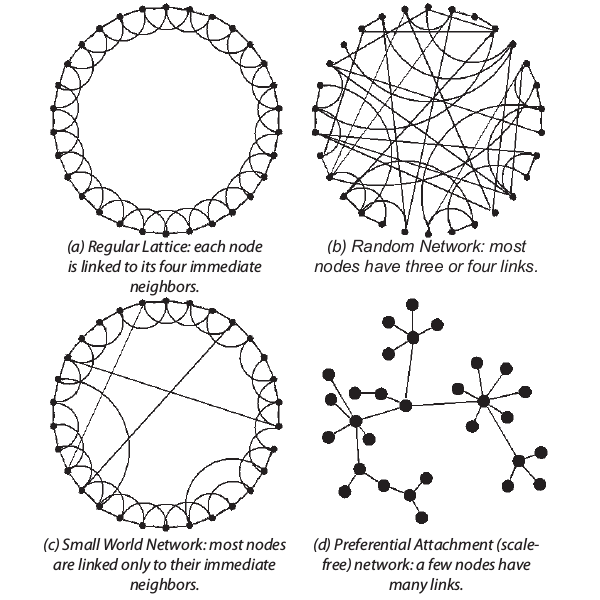
\includegraphics[scale=0.9]{images/Hamill_Gilbert11.png}
\caption{I quattro modelli di rete descritti in \cite{gilbert}}
\end{figure}
Gli autori indicano la costruzione \textit{scale-free} come la migliore tra le quattro, in quanto presenta tutte le caratteristiche elencate in precedenza, con l'eccezione dell'\textit{assortatività}, non particolarmente riflessa nel modello. Passano quindi all'esposizione della loro proposta, un modello ad agenti basato sul concetto di \textit{social circles} \cite{gilbert}: ogni agente può stabilire un ``link" con un altro agente solo se quest'ultimo può fare altrettanto. Quest'idea di \textit{reciprocità} si adatta bene alla modellazione di alcune piattaforme (es. Facebook), mentre si adatta meno su altre: un esempio è Twitter, dove per stabilire un collegamento, il fatto che due utenti si conoscano direttamente è poco rilevante. \\ \\
L'idea che una rete sociale sia assimilabile a una rete ad invarianza di scala (ovvero i cui nodi seguono una \textit{power law}, vedi \ref{subsec:graph}) è largamente supportata in letteratura: testi importanti e fondamentali come \cite{barabasi} e \cite{newman} asseriscono che i social network, così come il World Wide Web stesso, siano organizzati in modo tale che pochi nodi abbiano molti collegamenti e siano collegati tra di loro, mentre molti nodi abbiano pochi collegamenti e siano collegati ad alcuni di questi ``hub". Entrambi i testi, così come \cite{gilbert}, ricordano però l'assunzione \textit{small-world}, che, specialmente per i social network, debba essere verificata. 
\\
\\
Un altro lavoro che abbiamo recuperato è quello di Liben-Nowell \& Kleinberg \cite{link}. Il problema da loro affrontato è quello della previsione di collegamenti (\textit{link prediction}) nei social network, ovvero prevedere, dato lo stato del sistema in un dato istante di tempo, la formazione di nuovi collegamenti negli istanti immediatamente successivi. In una simulazione \textit{dinamica} di una rete è fondamentale stabilire un metodo per cui nuovi collegamenti vengono stabiliti tra i nodi. Un aspetto cruciale in questo caso è il criterio con cui viene valutata la \textit{similarità} tra i nodi del grafo, ovvero come viene assegnato uno \textit{score} a una coppia di nodi (arco) in modo che ne misuri la \textit{``distanza"} rispetto ad una particolare proprietà o caratteristica. Nodi simili ma non ancora collegati avranno infatti un'alta probabilità di stabilire un collegamento negli istanti di tempo più prossimi. \\
Nell'articolo viene fatta una rassegna dei metodi principali; l'obiettivo di questi metodi è costruire la matrice di similarità :
\begin{description}
\item[Neighborhood-based methods] Di questa categoria fanno parte tutti quei metodi che si basano sul \textit{vicinato} (\textit{neighborhood}) dei nodi di cui si vuole calcolare la similarità. La misura di distanza può essere il numero di nodi adiacenti in comune, oppure la probabilità che i due nodi in esame abbiano un vicino in comune, per esempio usando la \textit{distanza di Jaccard}. In alternativa, questa probabilità può essere calcolata in modo proporzionale alla dimensione dei vicinati dei due nodi candidati, per esempio moltiplicandone la cardinalità.
\item[Paths-based methods] Anche la distanza intesa come lunghezza di un cammino tra due nodi può essere intesa come misura di similarità; per esempio, in \cite{katz} viene descritta una metrica che prende in considerazione la lunghezza tutti i cammini esistenti tra due nodi per quantificarne la similarità. Anche alcuni celebri algoritmi, come il \textit{PageRank} di Google \cite{google}, fanno parte di questa categoria.
\end{description}
Altre tecniche possono essere usate in congiunzione con i metodi sopra elencati, per semplificarne la computazione oppure per irrobustirne la previsione. Procedure di \textit{clustering} o \textit{matrix factorization} possono aiutare ad eliminare i collegamenti meno significativi prima dell'effettivo calcolo delle metriche. \\
\\
Essendo però il nostro obiettivo la simulazione di una \textit{social} network, non si può ignorare la (forte) componente sociale del sistema considerato. Ogni nodo rappresenta un utente, e dunque ne eredita le caratteristiche personali come interessi e carattere. La letteratura specializzata in \textit{social sciences} ha da tempo definito il concetto di \textit{omofilia} (\textit{homophily}) \cite{homo} \cite{newman}, inteso come la tendenza di ogni individuo a stringere legami con altri individui dalle caratteristiche simili. Nel computo della misura di similarità (o dissimilarità) bisognerebbe quindi tenere conto di tali caratteristiche e trovare quindi il modo di rappresentarle nel sistema. In \cite{group}, per esempio, gli autori hanno tentato di tradurre in linguaggio matematico l'idea di omofilia, in particolare per quanto riguarda l'aggregazione di individui in base al gruppo di appartenenza. Dopo aver effettuato un'etichettatura degli individui in base a questi raggruppamenti, hanno definito un indice  $H_i$ per l'omofilia:
\begin{equation}
H_i = \dfrac{s_i}{s_i + d_i}
\end{equation}
dove $s_i$ indica il numero medio di \textit{amicizie} (\textit{friendships}) che un individuo facente parte del gruppo $i$ ha con i membri dello stesso gruppo, mentre $d_i$ indica il numero medio di \textit{amicizie} che un membro del gruppo $i$ ha con gli individui appartenenti ad altri gruppi. Questa misura, se confrontata con la frequenza relativa $w_i$ degli individui apparteneti al gruppo $i$, fornisce un indicazione del comportamento degli agenti all'interno del sistema, ovvero se tendono a stabilire conllegamenti fra individui dello stesso gruppo (\textit{inbreeding homophily}) oppure con individui apparteneti ad altri gruppi (\textit{heterophily}).\\
Occorre notare come, nell'ambito dei social network, il termine \textit{omofilia} e il termine \textit{assortatività} siano spesso indicati come sinonimi. \cite{assor} e \cite{mixing} per esempio, forniscono rispettivamente una misura di assortatività per attributo e per grado (vedi \ref{subsec:graph}), ovvero un indice di quanto i vertici di una rete siano legati a nodi con simili valori per l'attributo considerato oppure con simili gradi di archi entranti o uscenti.
\\
\\
Esistono modelli agent-based oltre a quello esposto in \cite{gilbert}, per esempio quelli descritti in \cite{red} e \cite{det}; entrambi usano una rete \textit{scale-free} come ambiente per gli agenti (il primo orientata, la seconda non orientata), ed entrambi regolano gli eventi che accadono nel sistema e le azioni degli agenti secondo degli spazi di probabilità, che si aggiornano dinamicamente. Queste probabilità sono in funzione dell'\textit{in-degree} di ogni nodo e della \textit{similarità} tra ogni coppia di nodi. In particolare, \cite{red} contempla anche l'aggiunta e la delezione di nodi durante la simulazione, operazioni anch'esse regolate da una specifica distribuzione di probabilità. \\
\\
Un'ultima risorsa da noi sfruttata è stata la relazione stilata da Marco Comi e Marco Gravina che, come noi e prima di noi, si sono cimentati nella simulazione del social network Twitter. Abbiamo preso spunto dalle loro soluzioni e dalle criticità del loro modello per sviluppare la nostra proposta.
\section{Riferimenti matematici}
Di seguito descriviamo brevemente alcuni concetti matematici fondamentali per la comprensione delle sezioni successive.
\label{sec:mat}
\subsection{Cosine similarity}
\label{subsec:cos}
Il \textit{coseno di similitudine} (\textit{cosine similarity}) \cite{ir} è una misura di similarità tra due vettori $v_1$ e $v_2$, definita in questo modo:
\begin{equation}
sim(v_1,v_2) = \dfrac{v_1v_2}{|v_1||v_2|}
\end{equation}
dove il numeratore rappresenta il \textit{prodotto scalare} tra i due vettori, mentra il denominatore rappresenta il prodotto dei moduli. I valori possibili ricandono nell'intervallo $[-1,1]$, dove $1$ si ottiene in caso di vettori identici, mentre $-1$ in caso di completa dissimilarità (vettori opposti). 
\subsection{Teoria dei grafi}
\label{subsec:graph}
Un \textit{grafo orientato} $G$ \cite{cormen} è una coppia $(V,E)$, dove $V$ (insieme dei \textit{vertici}) è un insieme finito ed $E$ è una relazione binaria in $V$.\\
Se $(u,v)$ è un arco \cite{cormen} di un grafo $G = (V,E)$ diciamo che il vertice $v$ è \textit{adiacente} al vertice $u$.\\
Dato un grafo $G$ orientato \cite{cormen}, il \textit{grado uscente} (\textit{out-degree}) di un vertice è il numero di archi che escono dal vertice; il \textit{grado entrante} (\textit{in-degree}) è il numero i archi che entrano nel vertice. \\
Un cammino (\textit{path}) \cite{barabasi} da un vertice $v_0$ a un vertice $v_n$ è una lista ordinata di archi $P = \{(v_0,v_1),(v_1,v_2),...,(v_{n-1},v_n)\}$, e $n$ corrisponde alla lunghezza di questo cammino. \\
\\
Un grafo orientato $G$ si dice \textit{completo} \cite{barabasi} quando ogni coppia di vertici è collegata da una coppia simmetrica di archi. La definizione è analoga al caso in cui il grafo sia non orientato, con la differenza che, in quest'ultimo, ogni coppia di archi opposti situata tra due nodi è sostituita da un solo arco non orientato. Il numero di archi \cite{barabasi} in un grafo \textit{non orientato completo} è pari a $\tfrac{N(N-1)}{2}$, dove $N$ è il numero di vertici del grafo. Se si escludono i \textit{cappi} (\textit{self-loops}), allora un grafo \textit{orientato completo} è composto da $N(N-1)$ archi. \\
\\
Si dice \textit{densità della rete} il rapporto tra il numero di archi esistenti e il numero di archi possibili (es. un grafo con densità al 50\% sarà composto da un numero di archi che è pari alla metà del totale di archi possibili).
\subsubsection{Coefficiente di clustering}
Il \textit{coefficiente di clustering} (\textit{clustering coefficient}) \cite{barabasi}, in un grafo \textit{non orientato}, cerca di esprimere il grado con cui i vicini di un dato nodo sono collegati tra di loro. Questo fornisce un'idea della compattezza del gruppo in cui è inserito quello specifico nodo. E' possibile inoltre avere una misura globale della tendenza dei nodi a ``raggrupparsi" calcolando il \textit{coefficiente di clustering medio} (\textit{average clustering coefficient}). Nei grafi orientati  \cite{newman} è disponibile una misura analoga, chiamata \textit{coefficiente di clustering globale} (\textit{global clustering coefficient}, a volte anche chiamata \textit{ratio of transitive triplets} \cite{barabasi}); la sua definizione è la seguente:
\begin{equation}
C_\Delta=\dfrac{3\times NumeroDiTriangoli}{NumberoDelleTripleConnesse}
\end{equation}
dove per \textit{triangolo} si intende un insieme di $3$ vertici, ognuno dei quali connesso agli altri due da archi, mentre per \textit{tripla connessa} si intende tre vertici $uvw$ connessi dagli archi $(u,v)$ e $(v,w)$. I valori possibili ricadono nell'intervallo $[0,1]$.
\subsubsection{Assortatività}
Una rete si dice \textit{assortativa} (\textit{assortative}) \cite{newman} se 
una frazione significativa dei suoi archi collegano vertici simili tra di loro. La similitudine può essere calcolata rispetto a un particolare attributo dei nodi, o, in alternativa, rispetto al \textit{grado} dei vertici. In quest'ultimo caso, in un grafo diretto \cite{assor} la \textit{in-assortativity} e la \textit{out-assortativity} misurano rispettivamente la tendenza dei nodi a legarsi con altri nodi che hanno \textit{in-degree} o \textit{out-degree} identico al loro. Sia $r()$ la funzione che calcola la assortatività, e siano indicati i due tipi di assortatività appena descritti come $r(in,in)$ e $r(out,out)$, è possibile estendere la portata della definizione definendo anche $r(in,out)$ e $r(out,in)$. Supponendo di voler calcolare $r(in,out)$, si ricorre alla seguente formula \cite{mixing}
\begin{equation}
r=\dfrac{\sum_{jk}jk(e_{jk}-q^{in}_jq^{out}_k)}{\sigma_{in}\sigma_{out}}
\end{equation}
dove $e_{jk}$ è la probabilità che un arco qualsiasi conduca da un nodo con \textit{in-degree} $j$ a un nodo con \textit{out-degree} $k$, $\sigma_{in}$ è la deviazione standard della distribuzione $q^{in}$ e $\sigma_{out}$ è la deviazione standard della distribuzione $q^{out}$. La distribuzione di probabilità $q^{out}_k$ (e analogamente $q^{in}_j$) è calcolata come segue:
\begin{equation}
q^{out}_k=\dfrac{(k+1)p^{out}_{k+1}}{\sum_kkp^{out}_k}
\end{equation}
dove $p^{out}_k$ è la probabilità che un nodo abbia \textit{out-degree} $k$. Al denominatore si trova l'out-degree medio della rete.
L'assortatività per attributo è analoga, e si calcola in questo modo:
\begin{equation}
r=\dfrac{\sum_{xy}xy(e_{xy}-a_xb_y)}{\sigma_a\sigma_b}
\end{equation}
dove $e_{xy}$ è la probabilità che un arco qualsiasi conduca da un nodo con valore dell'attributo $x$ a un nodo con valore $y$, mentre $a$ e $b$ sono rispettivamente le frequenze degli archi che escono ed entrano in un nodo con valori $x$ e $y$. In entrambi i casi il valore di $r$ ricade nell'intervallo $[-1,1]$, con $1$ a indicare la perfetta assortatività e $-1$ la perfetta disassortatività.   
\subsubsection{Rete a invarianza di scala}
Una rete viene indicata come \textit{rete a invarianza di scala} (\textit{scale free network}) se la distribuzione dei gradi dei nodi (probabilità $p(k_i)$ che un nodo scelto in modo random abbia grado $k_i$) segue una \textit{power law} \cite{scalefree}.\\
Una \textit{power law} \cite{barabasi} è una funzione $y=f(x)$ in cui il valore $y$ della funzione è proporzionale ad una potenza del valore in ingresso $x$:
\begin{equation}
p_x \sim x^{-\gamma}
\end{equation}
L'equazione 4 è chiamata \textit{power law distribution} e l'esopente $-\gamma$ è detto \textit{degree exponent}. La rappresentazione con il logaritmo dell'equazione 4 diventa
\begin{equation}
\log p_x \sim -\gamma \log p
\end{equation}
Se vale l'equazione 5, allora ci si aspetta che $\log p_x$ dipenda linearmente da $\log x$, con inclinazione della retta pari a $\gamma$, come indicato nella figura 2. Assumendo che il grado di un nodo sia una quantità discreta, si può adottare il formalismo per il discreto; in questo modo, l'equazione 4 diventa
\begin{equation}
p_x \sim Cx^{-\gamma}
\end{equation} 
dove $C$ è una costante.
\begin{figure}[h]
\centering
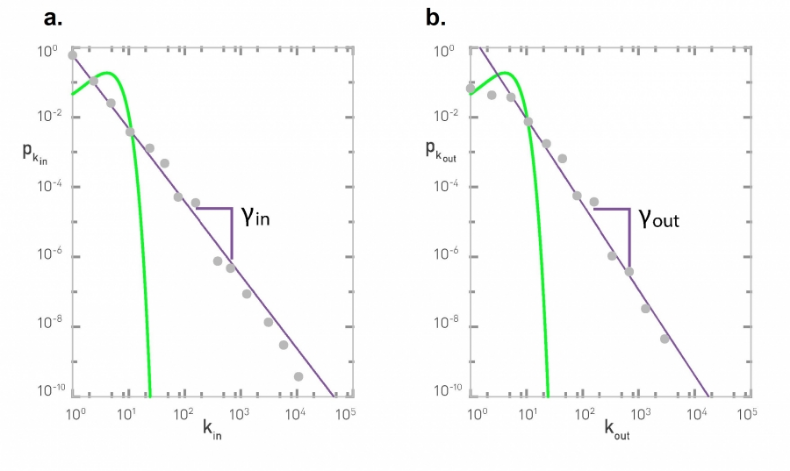
\includegraphics[scale=0.6]{images/powerlaw.png}
\caption{Distribuzione del WWW misurata nel 1999 \cite{barabasi}. La figura a. rappresenta la distribuzione dei nodi rispetto all'\textit{in-degree}, mentre b. rispetto all'\textit{out-degree}. Entrambe usano una scala logaritmica.}
\end{figure}
\section{Descrizione modello} 
\label{sec:mod}
\section{Visione multi-agente}
\label{sec:mas}
\section{Esperimenti}
\label{sec:esp}
In questa sezione esponiamo le prove condotte con il nostro modello. 
Abbiamo organizzato gli esperimenti in due fasi: 
\begin{description}
\item[Fase 1] Nella prima fase testiamo la solidità del nostro approccio andando a verificare che la rete rispetti le caratteristiche tipiche di una rete sociale.
\item[Fase 2] Nella seconda fase osserviamo il cambiamento del sistema all'occorrenza di un particolare evento, in particolare studiamo il ``salto" di popolarità da parte di un utente.
\end{description}
Per quanto riguarda la prima fase, uno dei rischi maggiori è produrre un modello incline al \textit{completamento della rete}, ovvero un modello i cui agenti, alla fine della simulazione, sono tutti collegati fra di loro da due archi (essendo un grafo diretto). In un social network reale questa cosa non si verifica, in quanto gli utenti non hanno interesse ad essere collegati con tutti gli altri. Questo è stato uno dei principali obiettivi durante la costruzione del modello, assieme alla conservazione della proprietà di \textit{invarianza di scala} e alla tendenza degli utenti a stabilire collegamenti secondo l'\textit{omofilia}. 
\\
\\
Nella seconda fase simuliamo lo scenario in cui un utente con pochi collegamenti in entrata, ovvero con pochi \textit{follower}, viene ``notato'' da uno degli ``hub", ovvero un utente con molti follower. Per far ciò, forziamo il retweet da parte dell'utente hub di un tweet creato ad-hoc per l'utente meno importante; dopodichè controlliamo la variazione di popolarità  dell'utente prescelto in termini di follower. Questo per simulare quanto avvenuto nel 2012 tra l'On. Maurizio Gasparri e l'utente Daniele Termite \cite{termite} dopo essere stato ``ripreso" su Twitter dall'Onorevole, l'utente Termite ha visto crescere improvvisamente di popolarità il suo account, con un boom di follower nel giro di brevissimo tempo, per poi assestarsi su un numero di circa 10.000 seguaci. La replica \textit{in-silico} di questo fenomeno utilizzando il nostro modello può essere considerata come indica di affidabilità dello stesso.
\\
\\
Per la realizzazione del modello e la conduzione degli esperimenti la scelta implementativa è ricaduta su \textit{Python} (versione 3) e sulla libreria \textit{networkx} \cite{nx}, un package molto curato e completo per la modellazione di reti. In principio avevamo optato per l'ambiente di simulazione PyCx, che fornisce un'interfaccia per la conduzione di esperimenti e la visualizzazione dei risultati, ma abbiamo riscontrato successivamente una incidenza negativa sulle performances del modello; per cui abbiamo virato su una CLI per l'inserimento dei parametri. La visualizzazione dei grafi è stata effettuata con il software Gephi, mentre i grafici delle metriche con R.
\subsection{Fase 1}
Per valutare la buona riuscita degli esperimenti, considerando quanto prodotto dalla letteratura, abbiamo individuato come parametri principali per valutare l'attendibilità della rete prodotta dal nostro modello le seguenti metriche:
\begin{enumerate}
    \item La \textit{densità} della rete, per monitorare la tendenza del modello al completamento o meno della rete.
    \item I parametri della \textit{power law} che intercorre sul grado dei nodi, per studiarne l'invarianza di scala.
\end{enumerate}
Altre metriche che abbiamo incluso nell'analisi sono:
\begin{enumerate}
    \item Il \textit{coefficiente di clustering}, per valutare la predisposizione alla formazione di gruppi di agenti.
    \item L'\textit{assortatività per attributo}, per valutare l'omofilia rispetto ai topic caratterizzanti gli utenti
    \item L'\textit{assortatività per grado r(out,in)}, a supporto del punto 2 della lista precedente, ovvero la valutazione dell'invarianza di scala.
    \item Il \textit{cammino minimo medio} (in caso di reti connesse) per verificare l'ipotesi di \textit{small world}
\end{enumerate}
Abbiamo quindi organizzato una sessione di esperimenti con i seguenti parametri comuni:
\begin{itemize}
\item 1000 utenti
\item 10 topic per utente
\item 1080 iterazioni (equivalenti a 90 giorni)
\end{itemize}
La differenza tra le varie run sta nella diversa istanziazione della rete iniziale; non avendo indicazioni sul valore di densità del grafo reale di Twitter, abbiamo optato per due soluzioni principali:
\begin{itemize}
\item Istanziazione di una rete scale-free, a densità fissa
\item Istanziazione di una rete random, a densità variabile
\end{itemize}
Il package networkx di Python permette l'istanziazione di una rete scale-free con una densità non modificabile pari a circa $0.1\%$: questo è dovuto al particolare modello usato dalla libreria, descritto in \cite{sfnx}, che per rispetto alla power law non permette la scelta del numero di archi iniziale.
A questa abbiamo quindi affincato una serie di prove con una random network come configurazione di partenza, avente valori diversi come densità iniziale: nello specifico, i valori sono $0.1\%$, $0.5\%$, $1.0\%$ e $5.0\%$.
\subsubsection{Risultati}
Le figure 3, 4, 5, 6 e 7 mostrano l'andamento dei quattro indici che abbiamo scelto per la valutazione.
\begin{figure}[h]
\begin{tabular}{cc}
  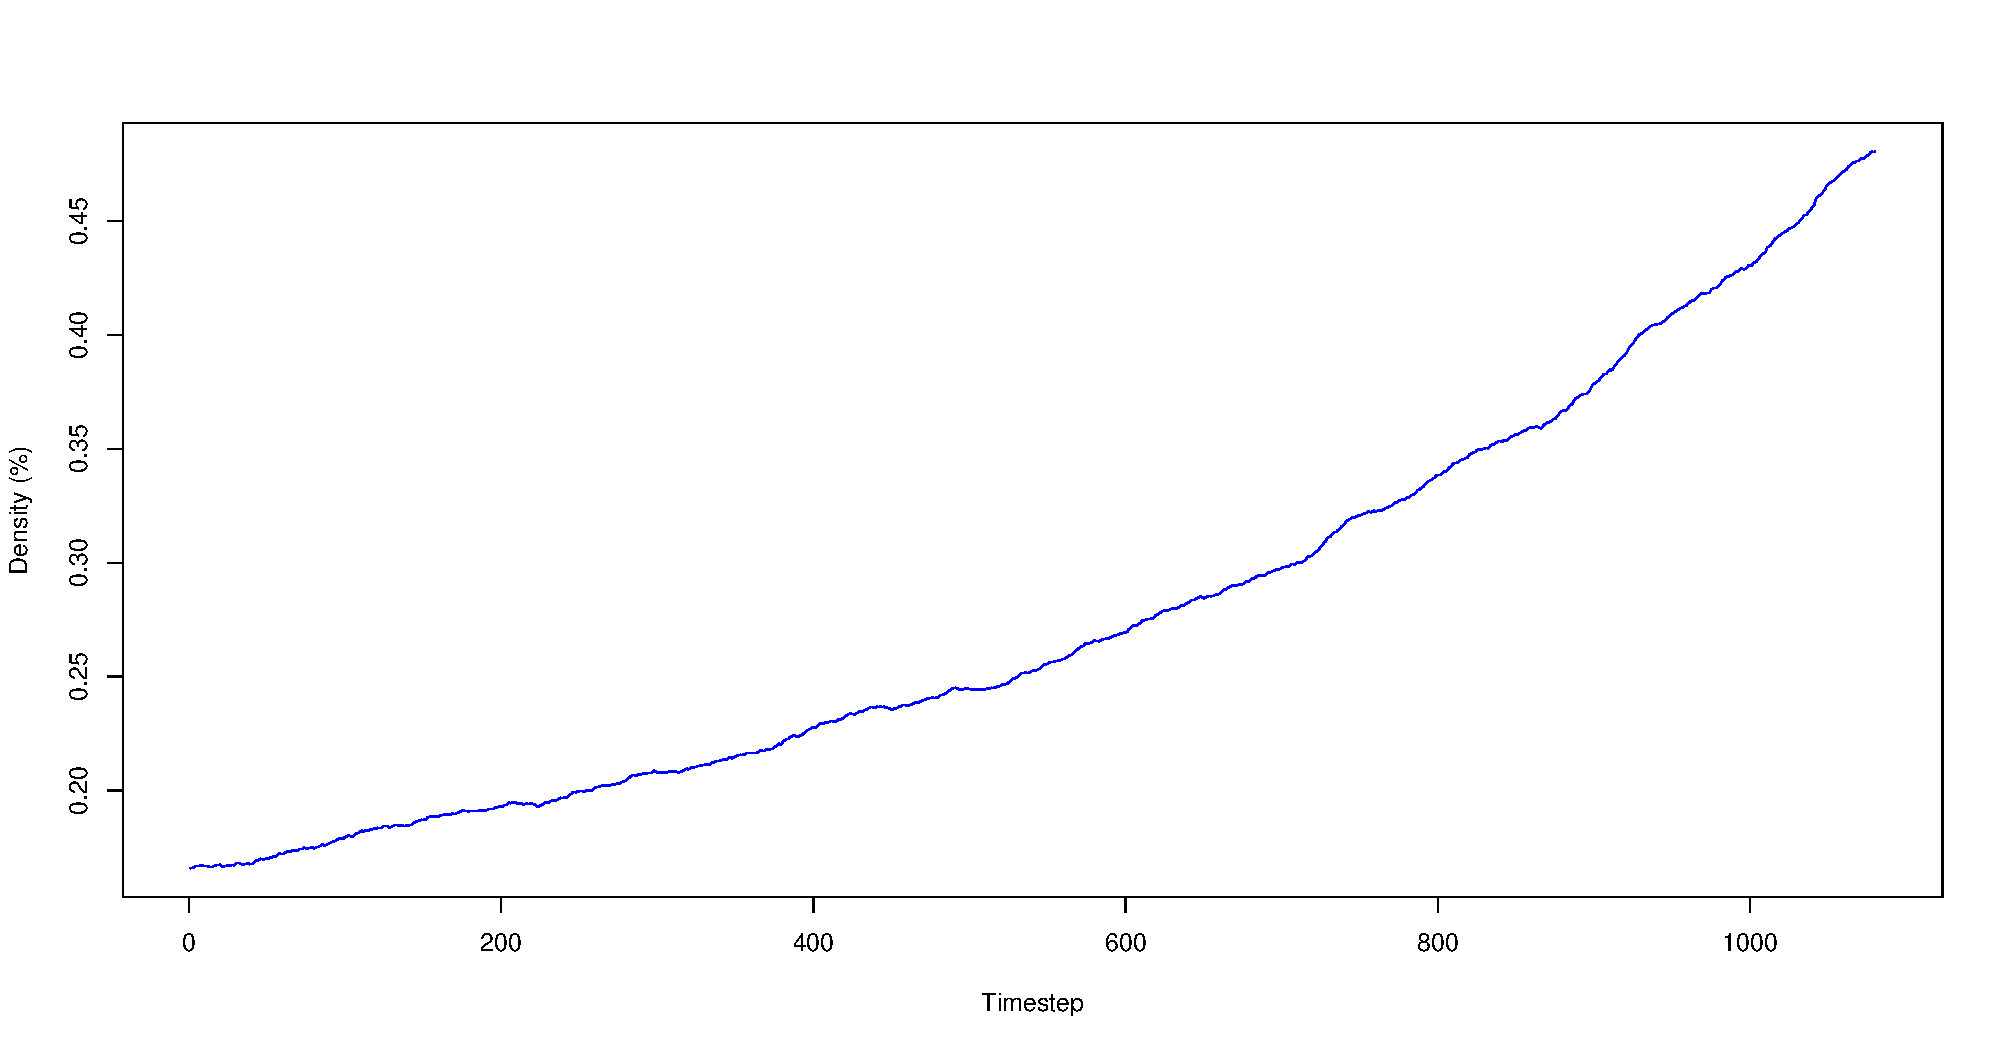
\includegraphics[width=83mm]{images/evolution_1000_sf_1080_0.pdf} &   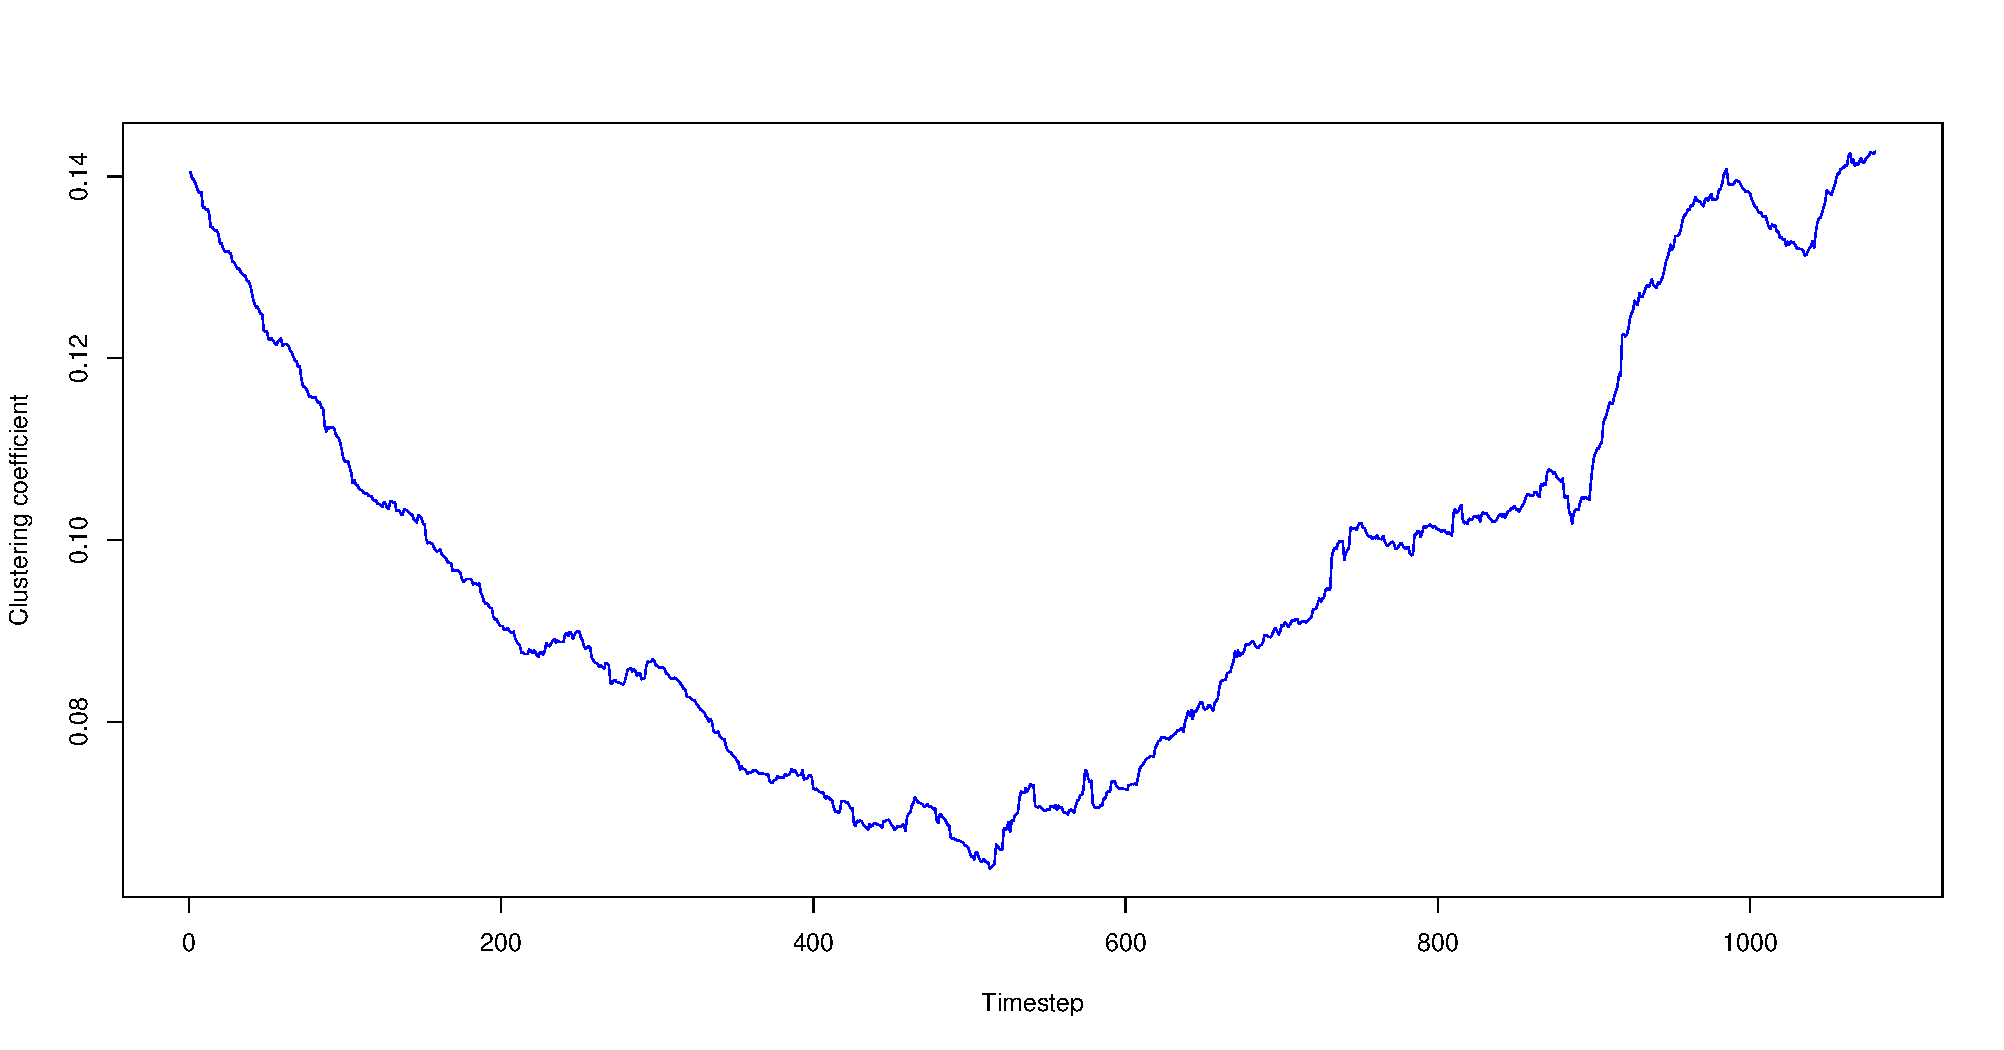
\includegraphics[width=83mm]{images/clustering_1000_sf_1080_0.pdf} \\
a. Densità & b. Coefficiente di clustering \\[6pt]
 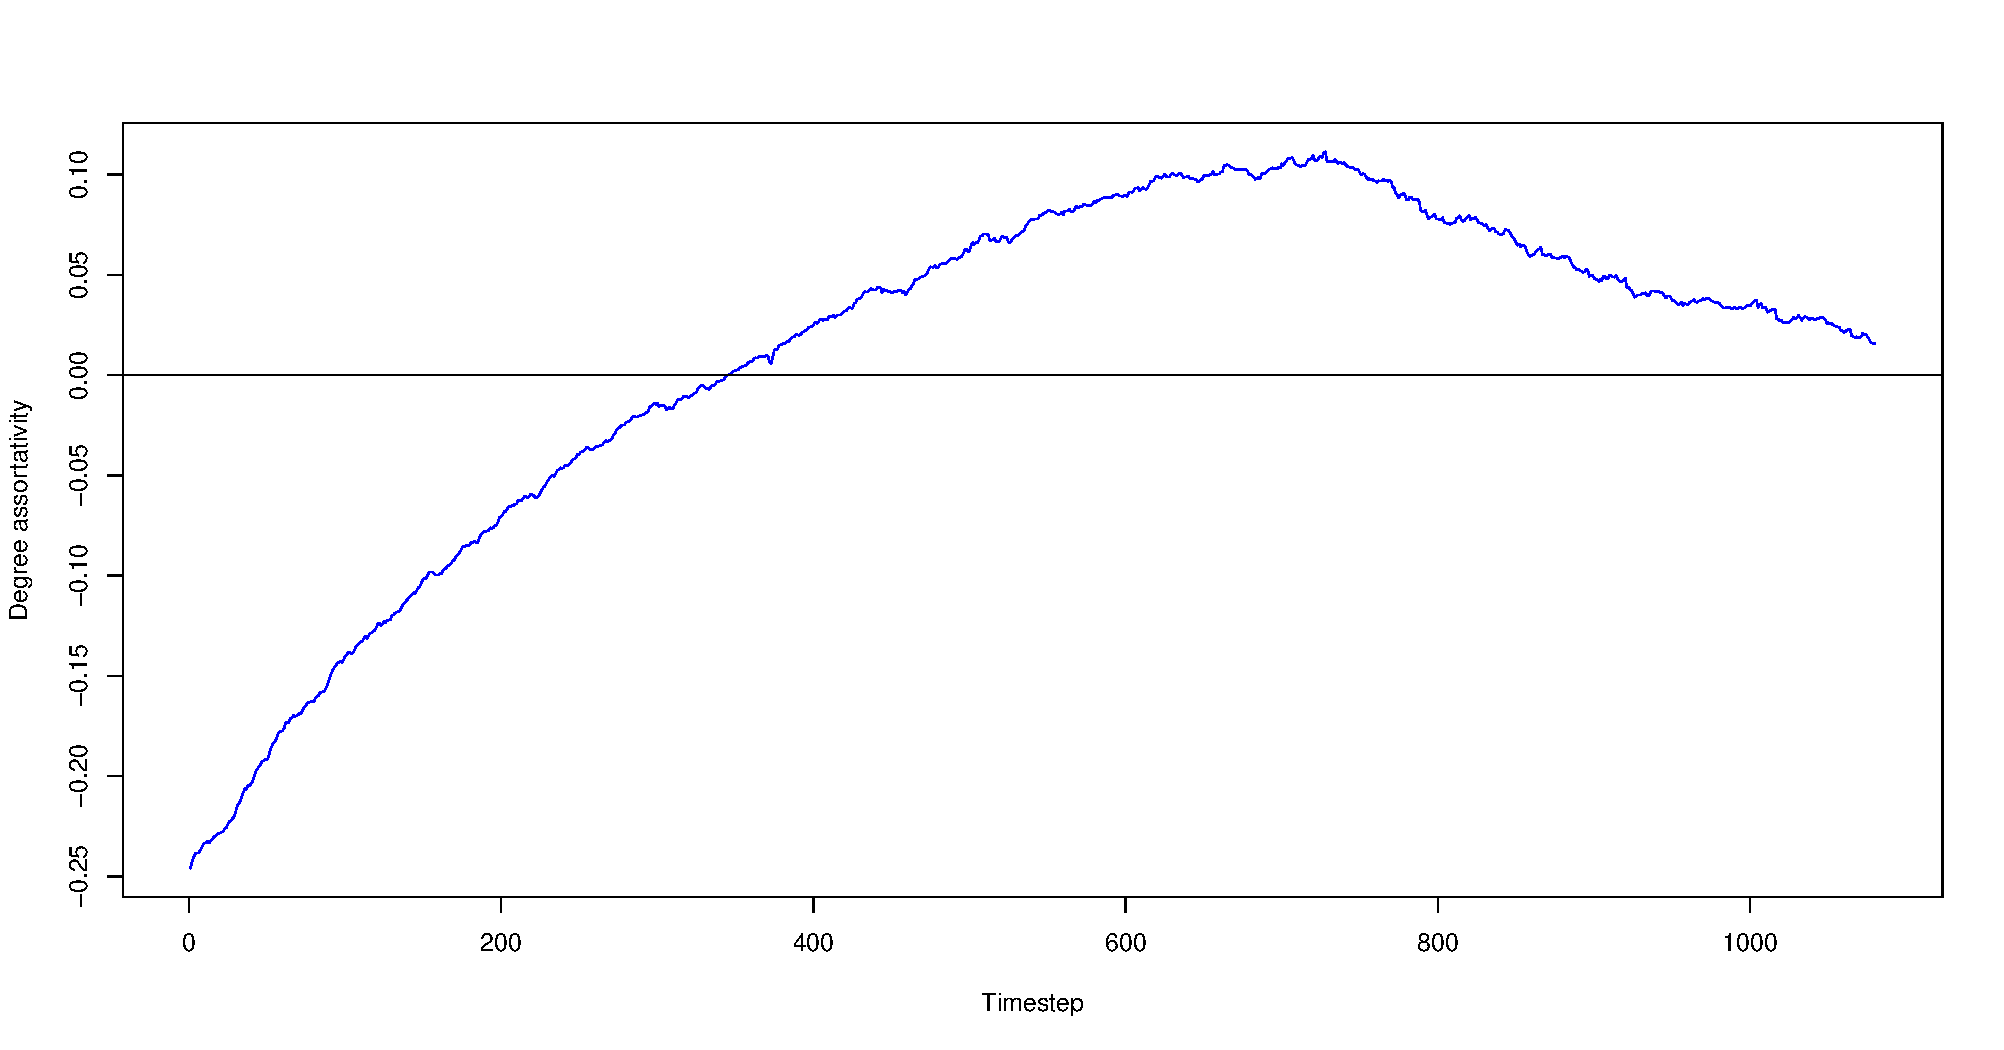
\includegraphics[width=83mm]{images/deg_assortativity_1000_sf_1080_0.pdf} &   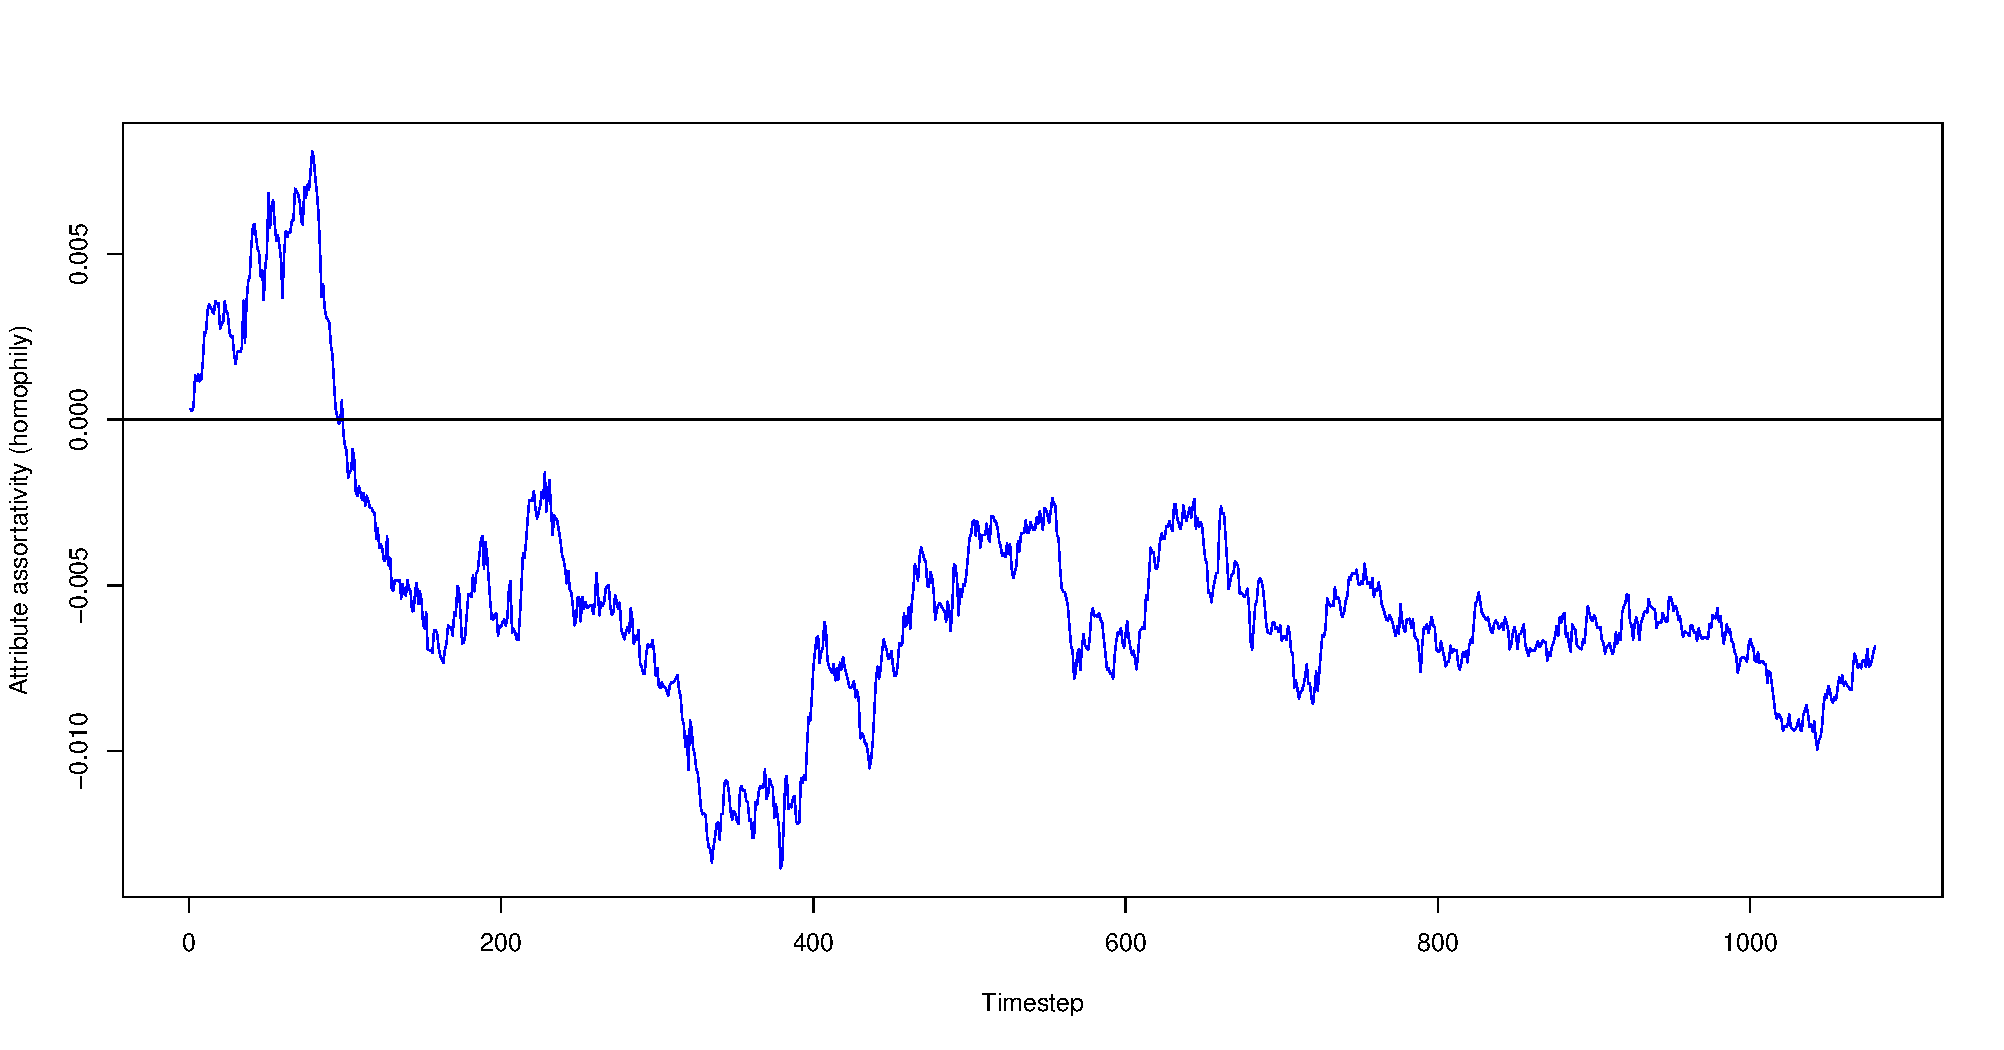
\includegraphics[width=83mm]{images/homophily_1000_sf_1080_0.pdf} \\
c. Assortatività per grado & d. Assortatività per attributo \\[6pt]
\end{tabular}
\caption{Indici scale-free network, densità 0.1\%}
\end{figure}
Nell'esperimento con istanziazione della rete iniziale a invarianza di scala (figura 3) si può notare come la densità cresca in modo piuttosto contenuto sebbene in modo debolmente esponenziale: da una densità iniziale di circa $0.1\%$ si arriva a circa $0.5\%$. Il coefficiente di clustering invece ha un andamento particolare: decresce fino a poco prima della metà del periodo considerato, per poi iniziare una crescita irregolare fino alla fine dell'esperimento. Una spiegazione di questo fenomeno potrebbe essere il fatto che, in principio, la rete abbia molti nodi senza alcun collegamento in entrata o in uscita; inoltre, una porzione ancora maggiore di questi nodi ha solo pochi collegamenti in uscita verso i due, tre nodi ``hub" che fanno capo alla maggior parte degli archi. \'E plausibile quindi che, fino ad un certo punto, i collegamenti non vadano a rafforzare comunità già presenti, quanto a unire per la prima volta nodi distanti.
Al contrario, l'assortatività per grado cresce regolarmente fino all'iterazione 750 circa, per poi cominciare a calare leggermente: questo è indice del fatto che a partire da quel momento, l'in-degree medio dei nodi con molti collegamenti cresce in modo più rapido dell'out-degree dei nodi con pochi collegamenti, con effetto negativo sulla misura di assortatività \textit{r(out,in)}. \\
A differenza degli altri indici, l'assortatività per attributo è molto irregolare: dopo un brusco calo che la porta ad assumere valori negativi, continua ad oscillare in prossimità dello zero, senza mai tornare a valori positivi. Questo è segno che i nodi tendono a formare legami a prescindere dal 
\begin{figure}[t]
\begin{tabular}{cc}
  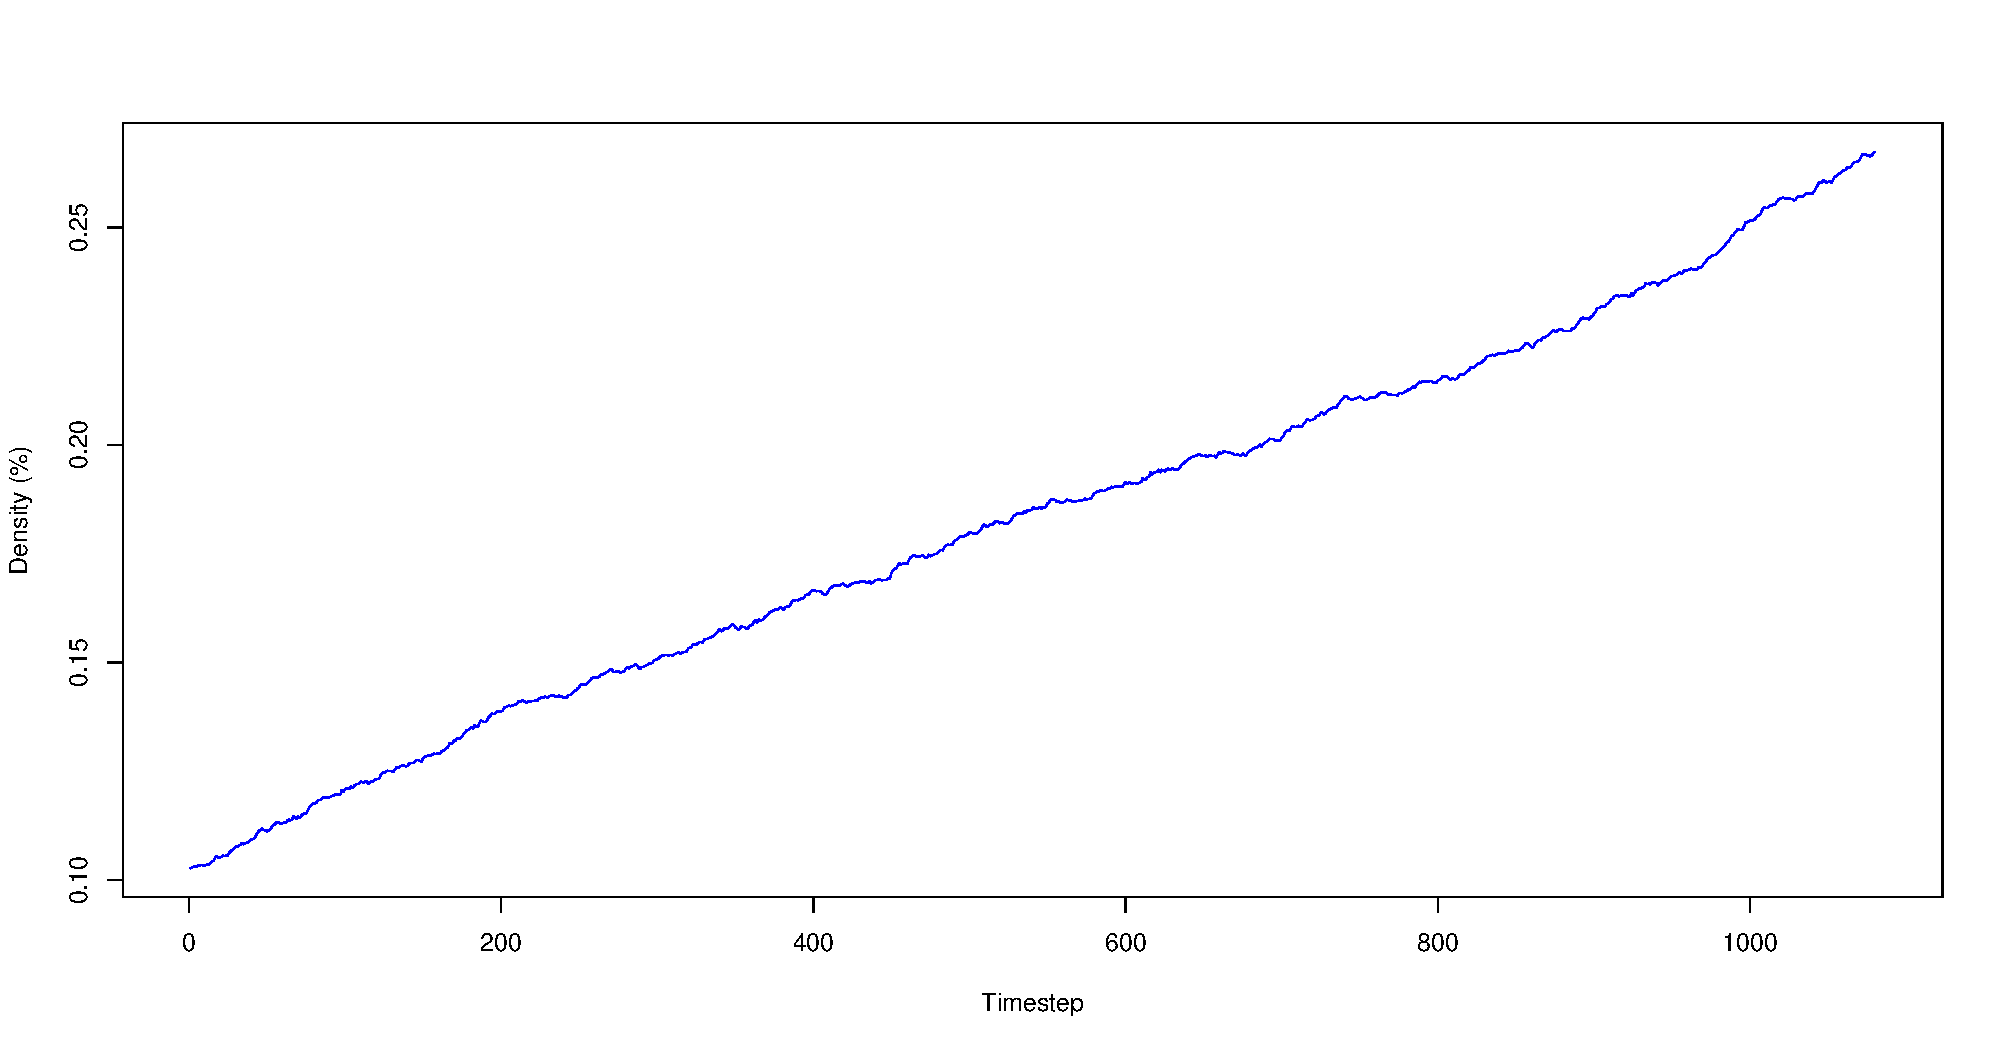
\includegraphics[width=83mm]{images/evolution_1000_rnd_1080_01_0.pdf} &   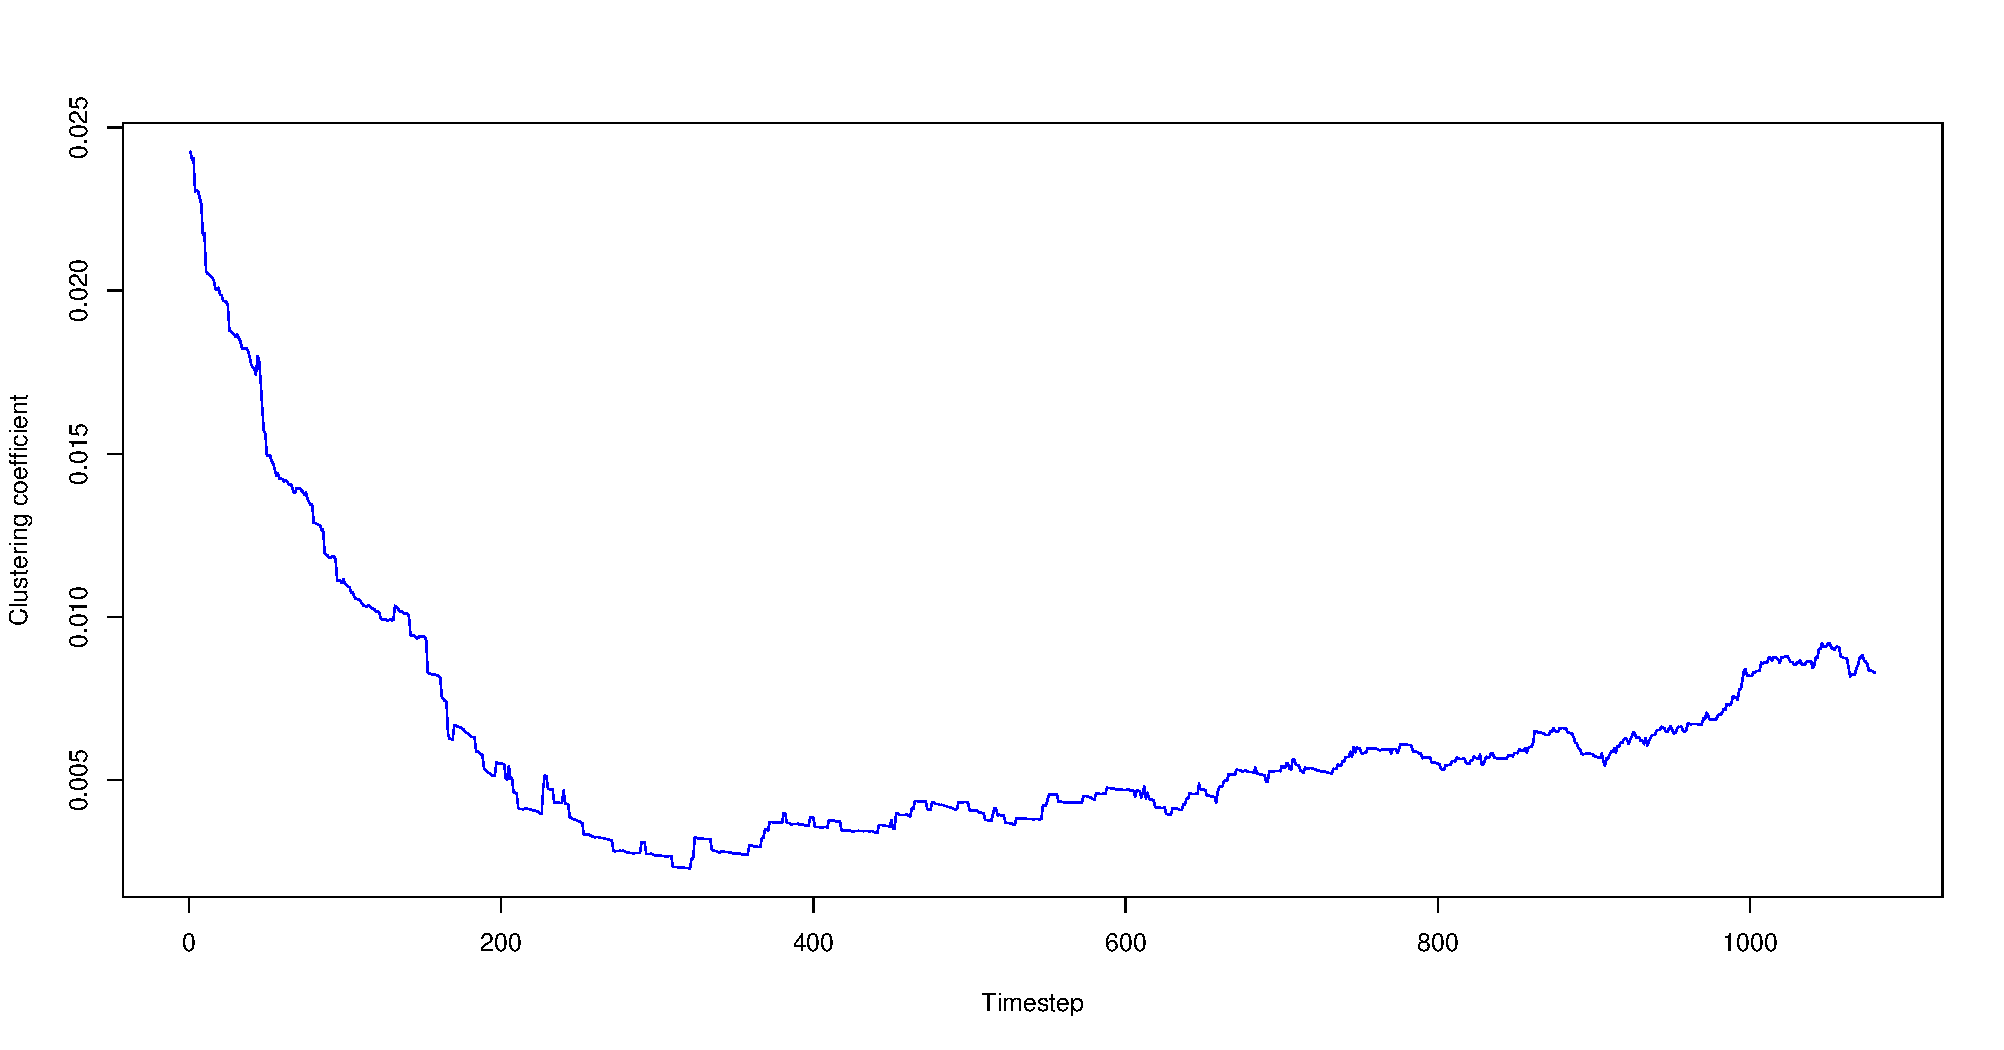
\includegraphics[width=83mm]{images/clustering_1000_rnd_1080_01_0.pdf} \\
a. Densità & b. Coefficiente di clustering \\[6pt]
 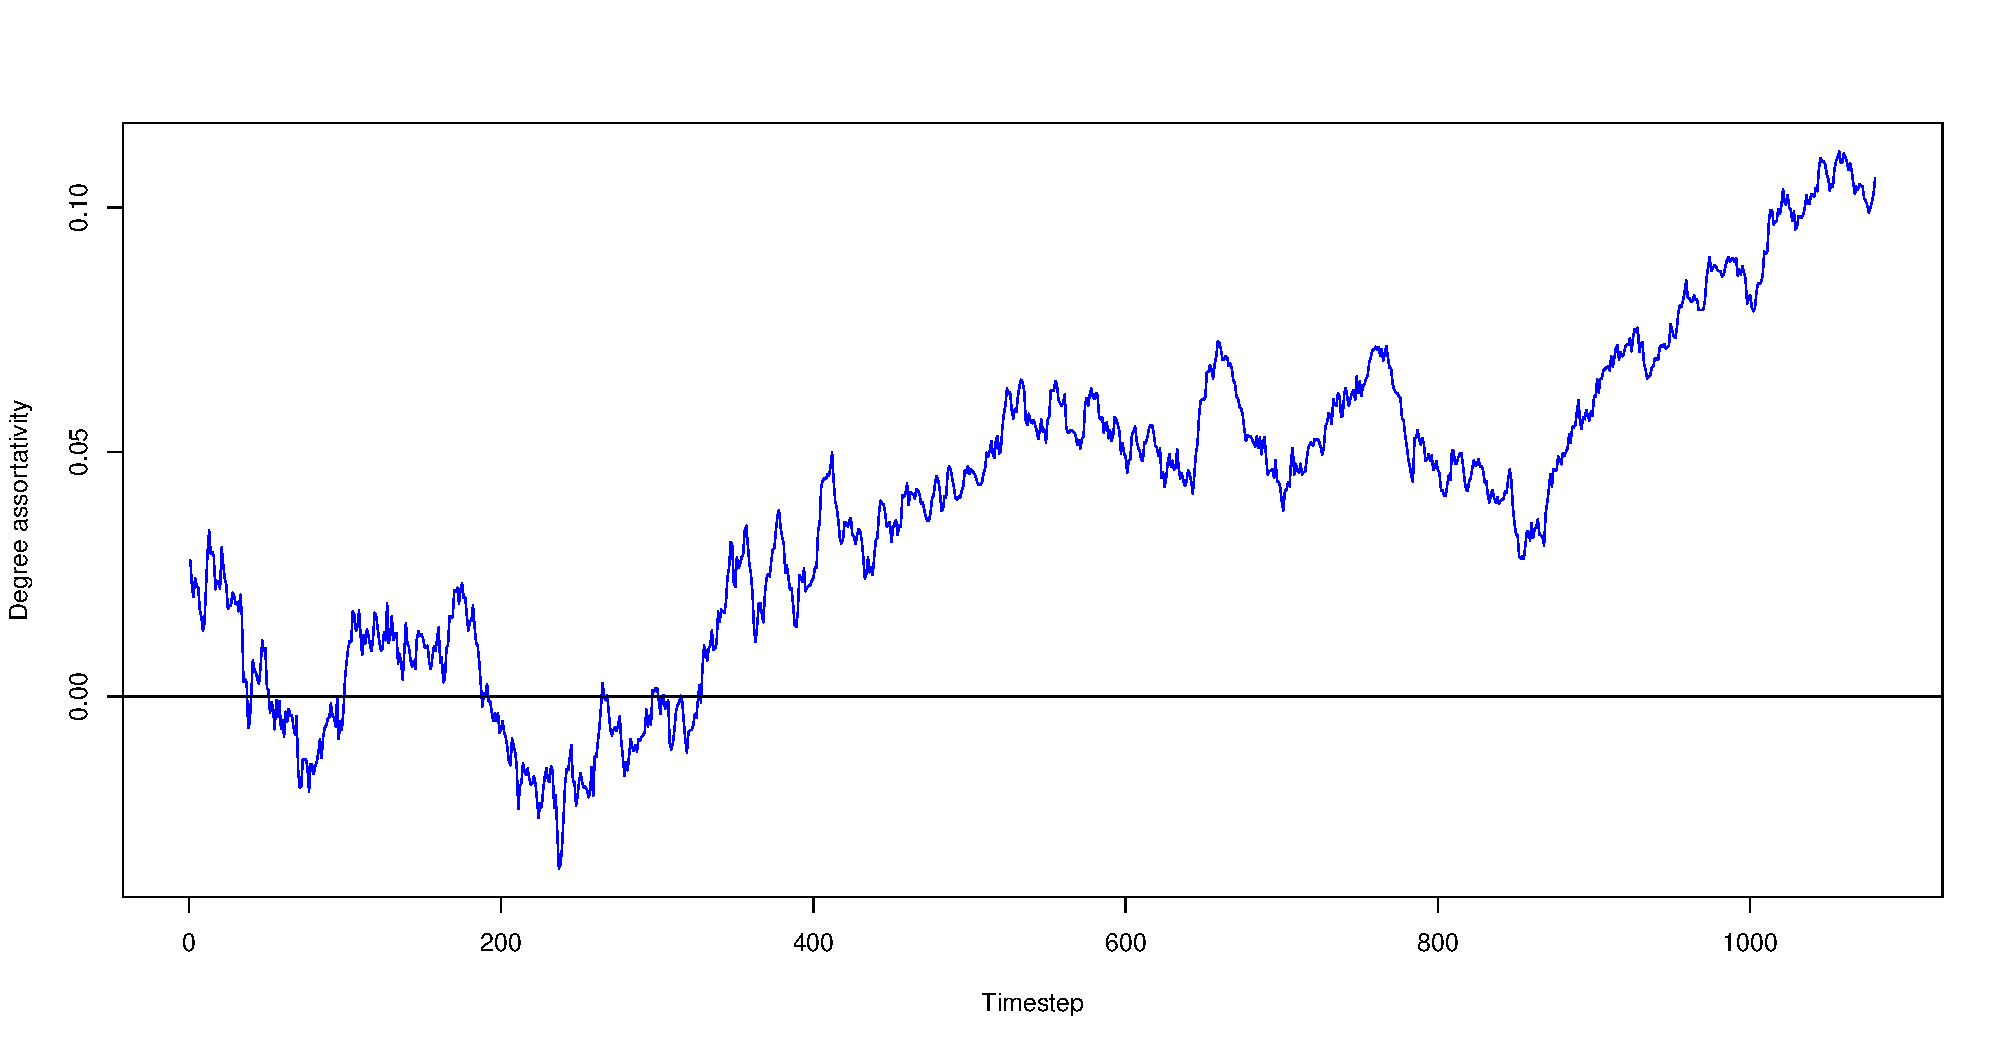
\includegraphics[width=83mm]{images/deg_assortativity_1000_rnd_1080_01_0.pdf} &   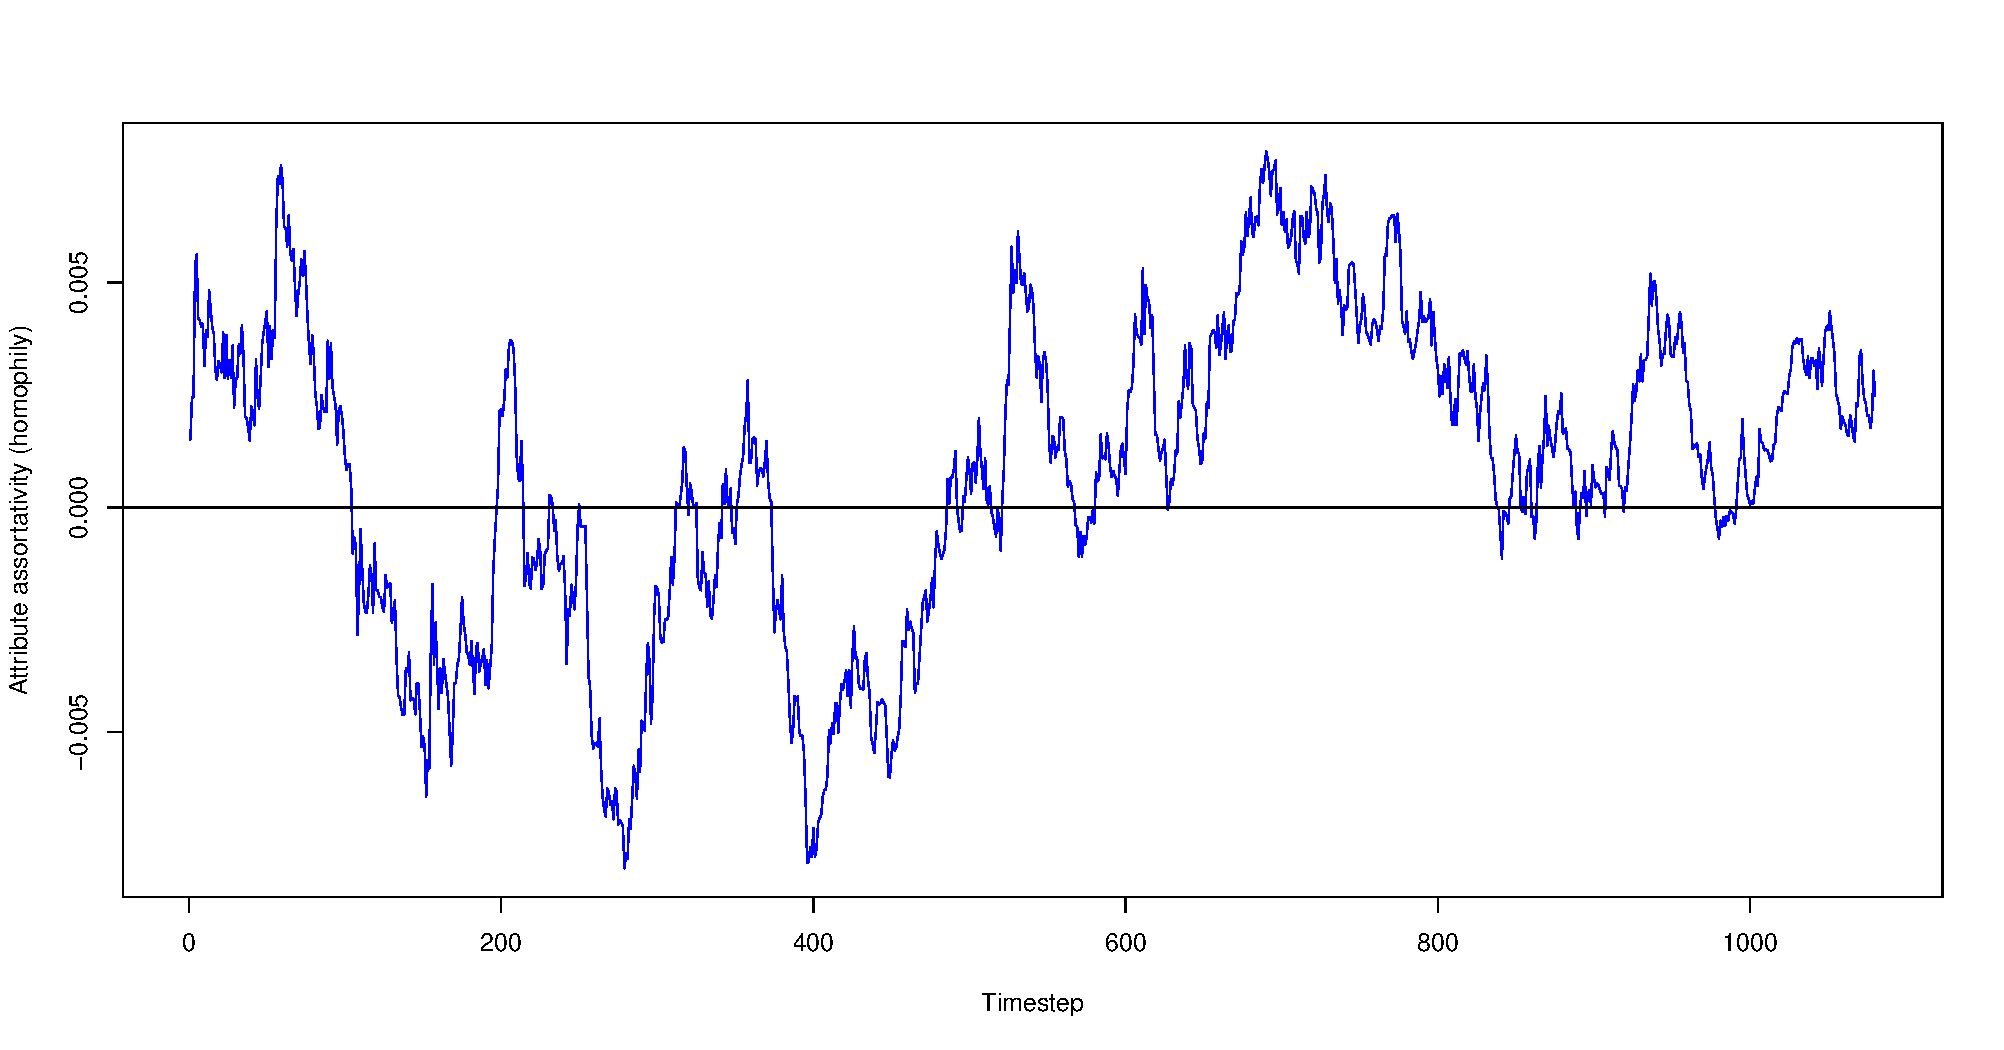
\includegraphics[width=83mm]{images/homophily_1000_rnd_1080_01_0.pdf} \\
c. Assortatività per grado & d. Assortatività per attributo \\[6pt]
\end{tabular}
\centering
\caption{Indici random network, densità 0.1\%}
\end{figure}
topic più rappresentativo di ognuno.\\ \\
L'esperimento successivo (figura 4) condivide con il primo il valore di densità iniziale, mentre differisce per costruzione: è infatti una random network priva, quindi, di nodi ``hub"; si riscontrano comunque nodi con più collegamenti in entrata e in uscita rispetto agli altri, ma la differenza, in questi termini, è molto ridotta. Ciò si rispecchia in una crescita molto più contenuta e lineare della densità (si arriva all'ultima iterazione con circa lo $0.3\%$), con i nodi che, avendo tutti un \textit{field of view} limitato, fanno fatica a stabilire nuovi collegamenti con nodi affini dal punto di vista degli interessi. Da qui si può trarre la conclusione che la presenza di nodi ``popolari" faciliti l'instaurazione di nuovi legami tra nodi meno importanti.
Inoltre, nell'andamento del coefficiente di clustering, si riscontra lo stesso fenomeno osservato in precedenza sulla scale-free network: dopo un calo iniziale, l'indice torna a crescere, ma in modo sensibilmente più lento rispetto all'altro caso. Da notare anche il valore di partenza, circa cinque volte minore. Anche questo comportamento può essere imputato alla scarsa densità e all'elevata sparsità degli archi, per cui le comunità vengono costituite con fatica. L'assortatività per grado mostra un andamento incerto ma crescente, a indicare che i nodi tendono a legarsi in base alla similarità tra out e in degree. L'assortatività per attributo è più incerta rispetto al caso precedente, con la differenza che nella seconda metà della simulazione rimane quasi sempre positiva.
\begin{figure}[h]
\begin{tabular}{cc}
  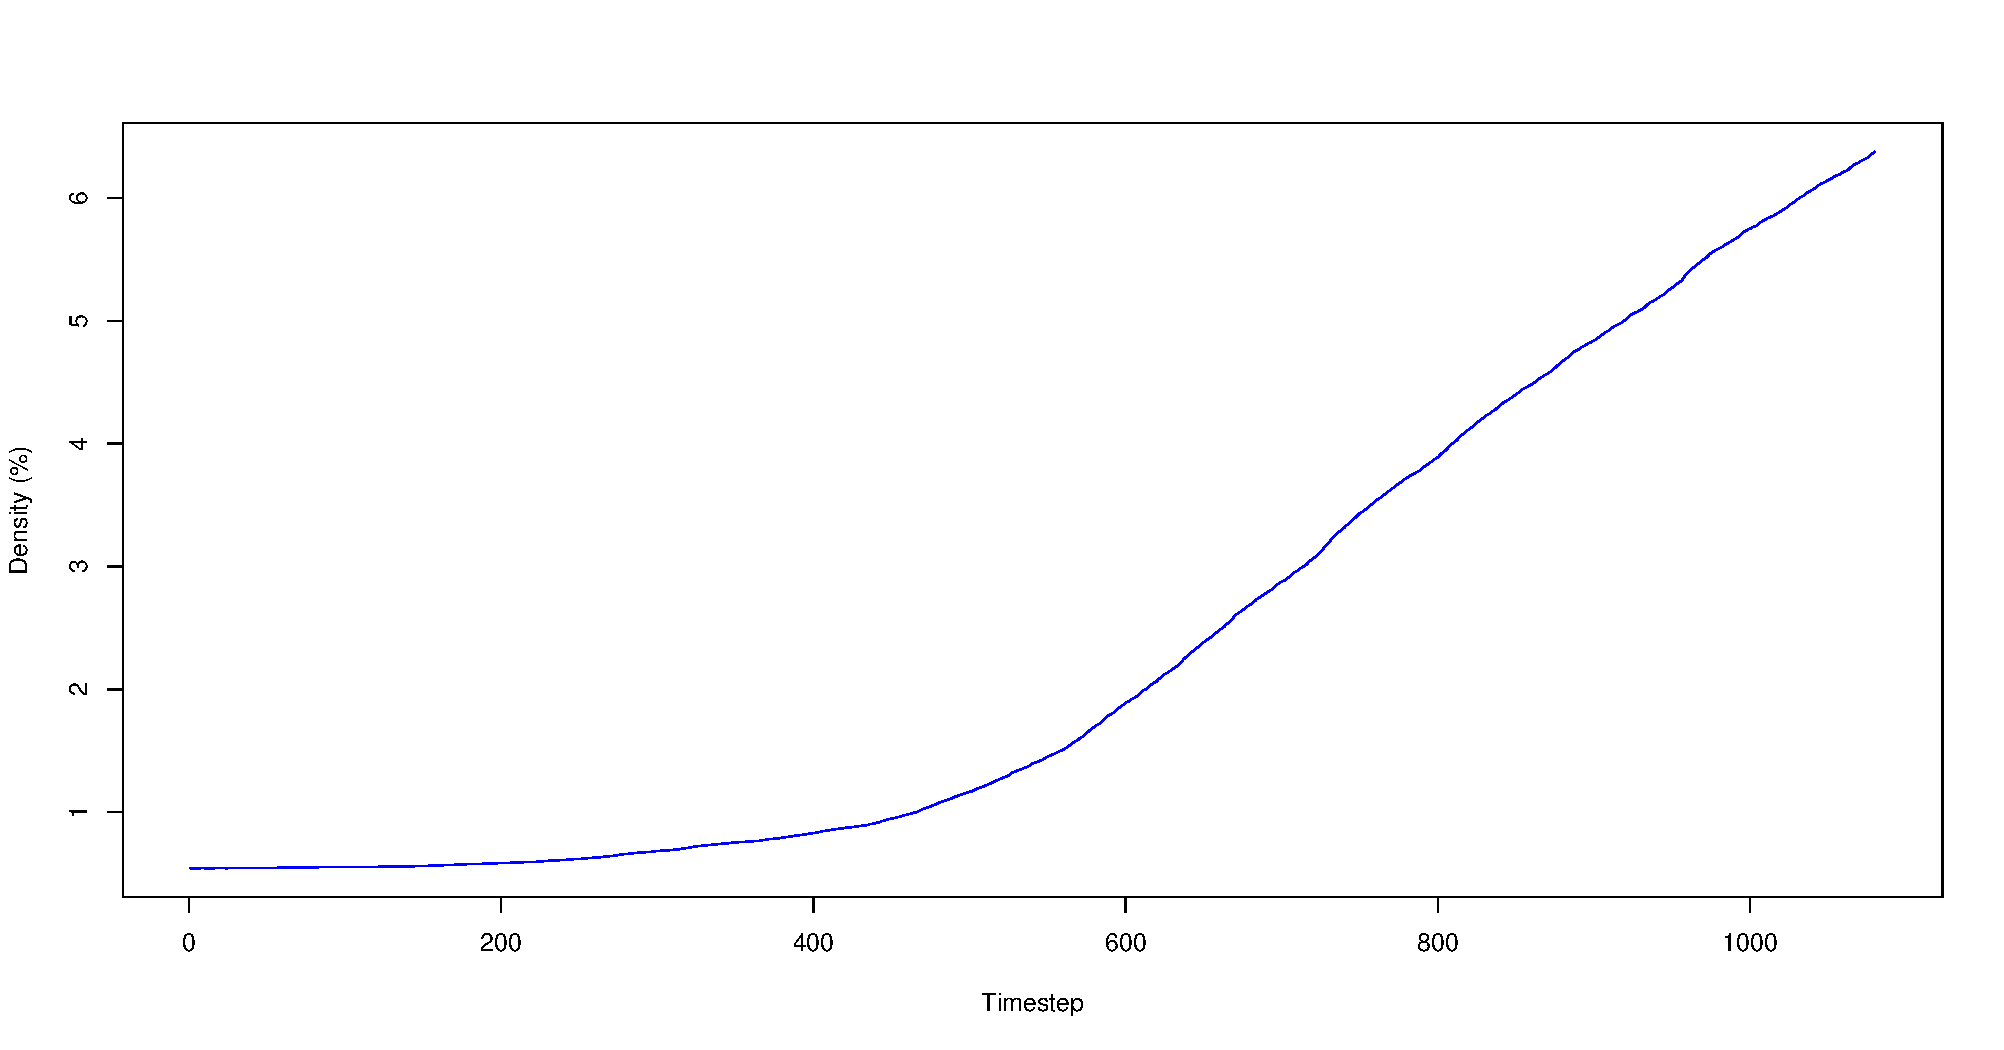
\includegraphics[width=81mm]{images/evolution_1000_rnd_1080_05_0.pdf} &   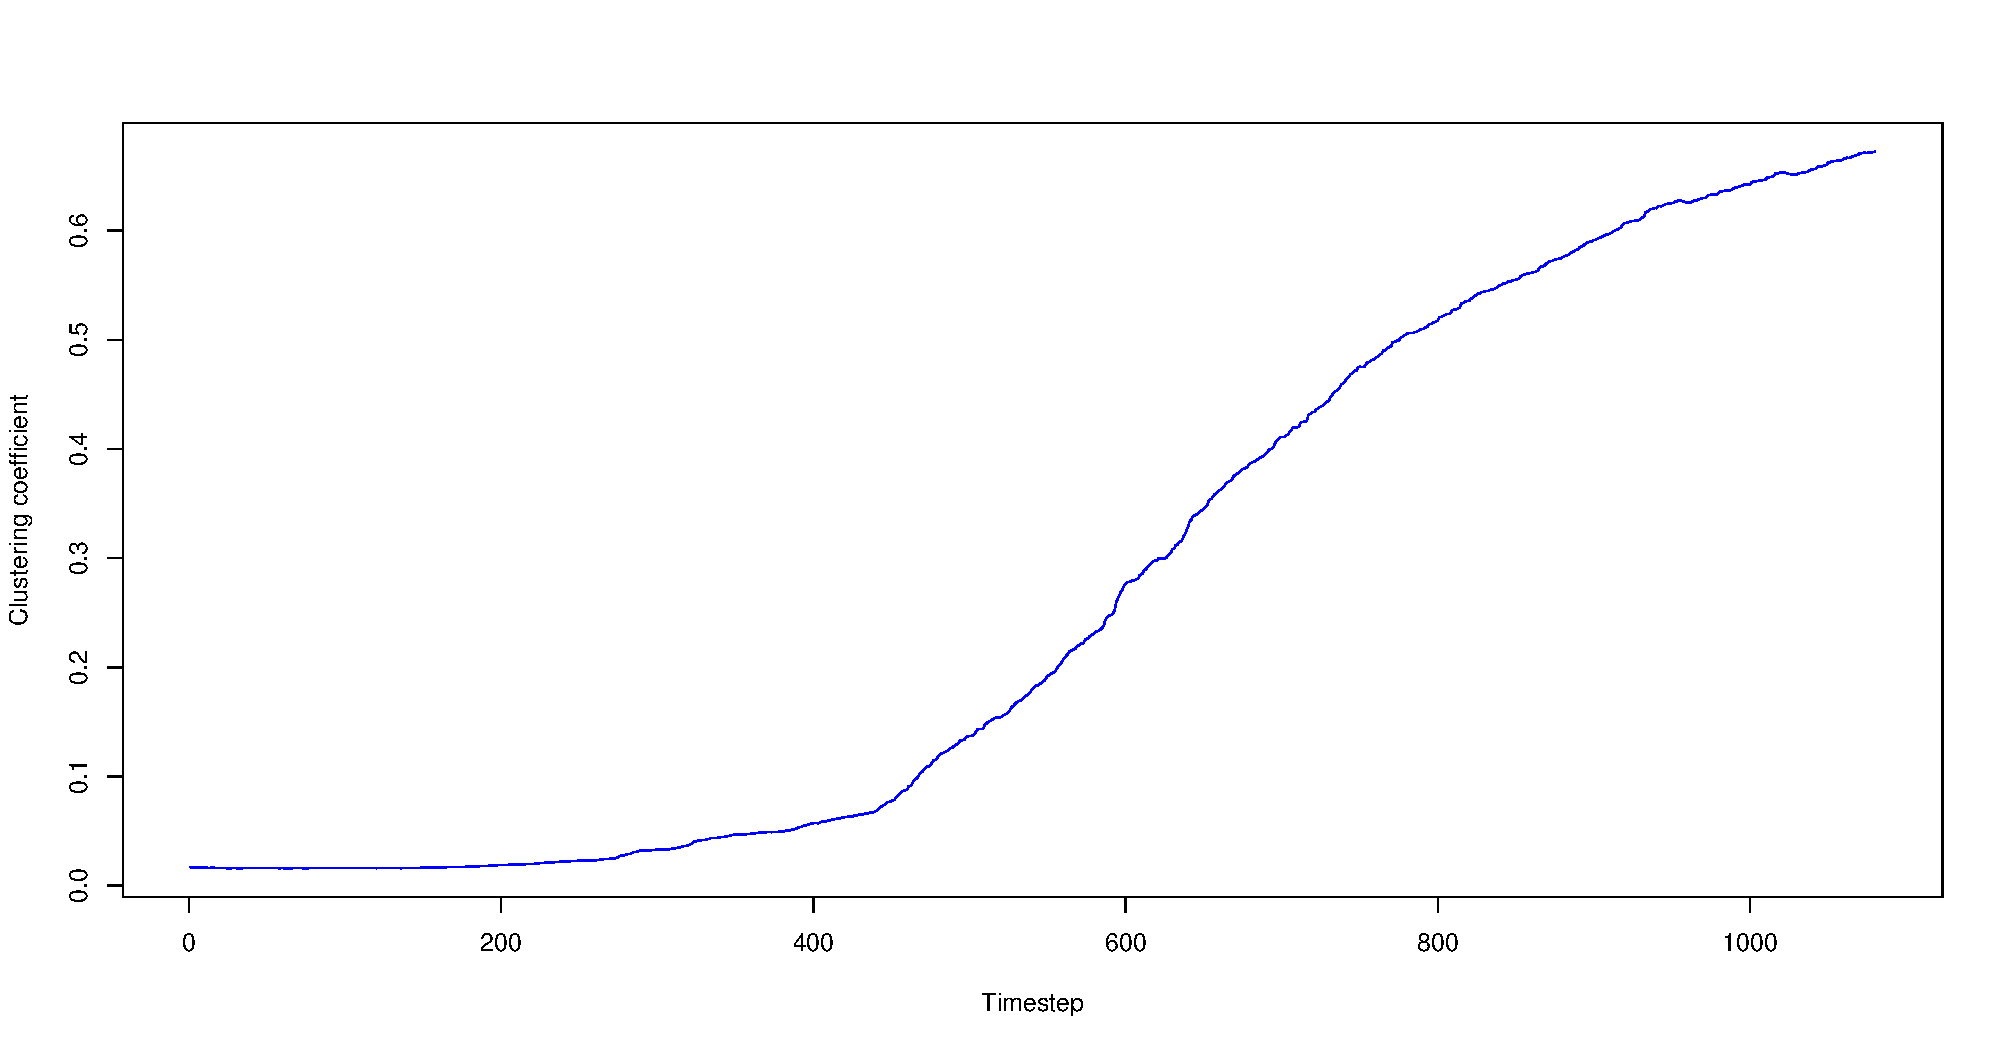
\includegraphics[width=81mm]{images/clustering_1000_rnd_1080_05_0.pdf} \\
a. Densità & b. Coefficiente di clustering \\[6pt]
 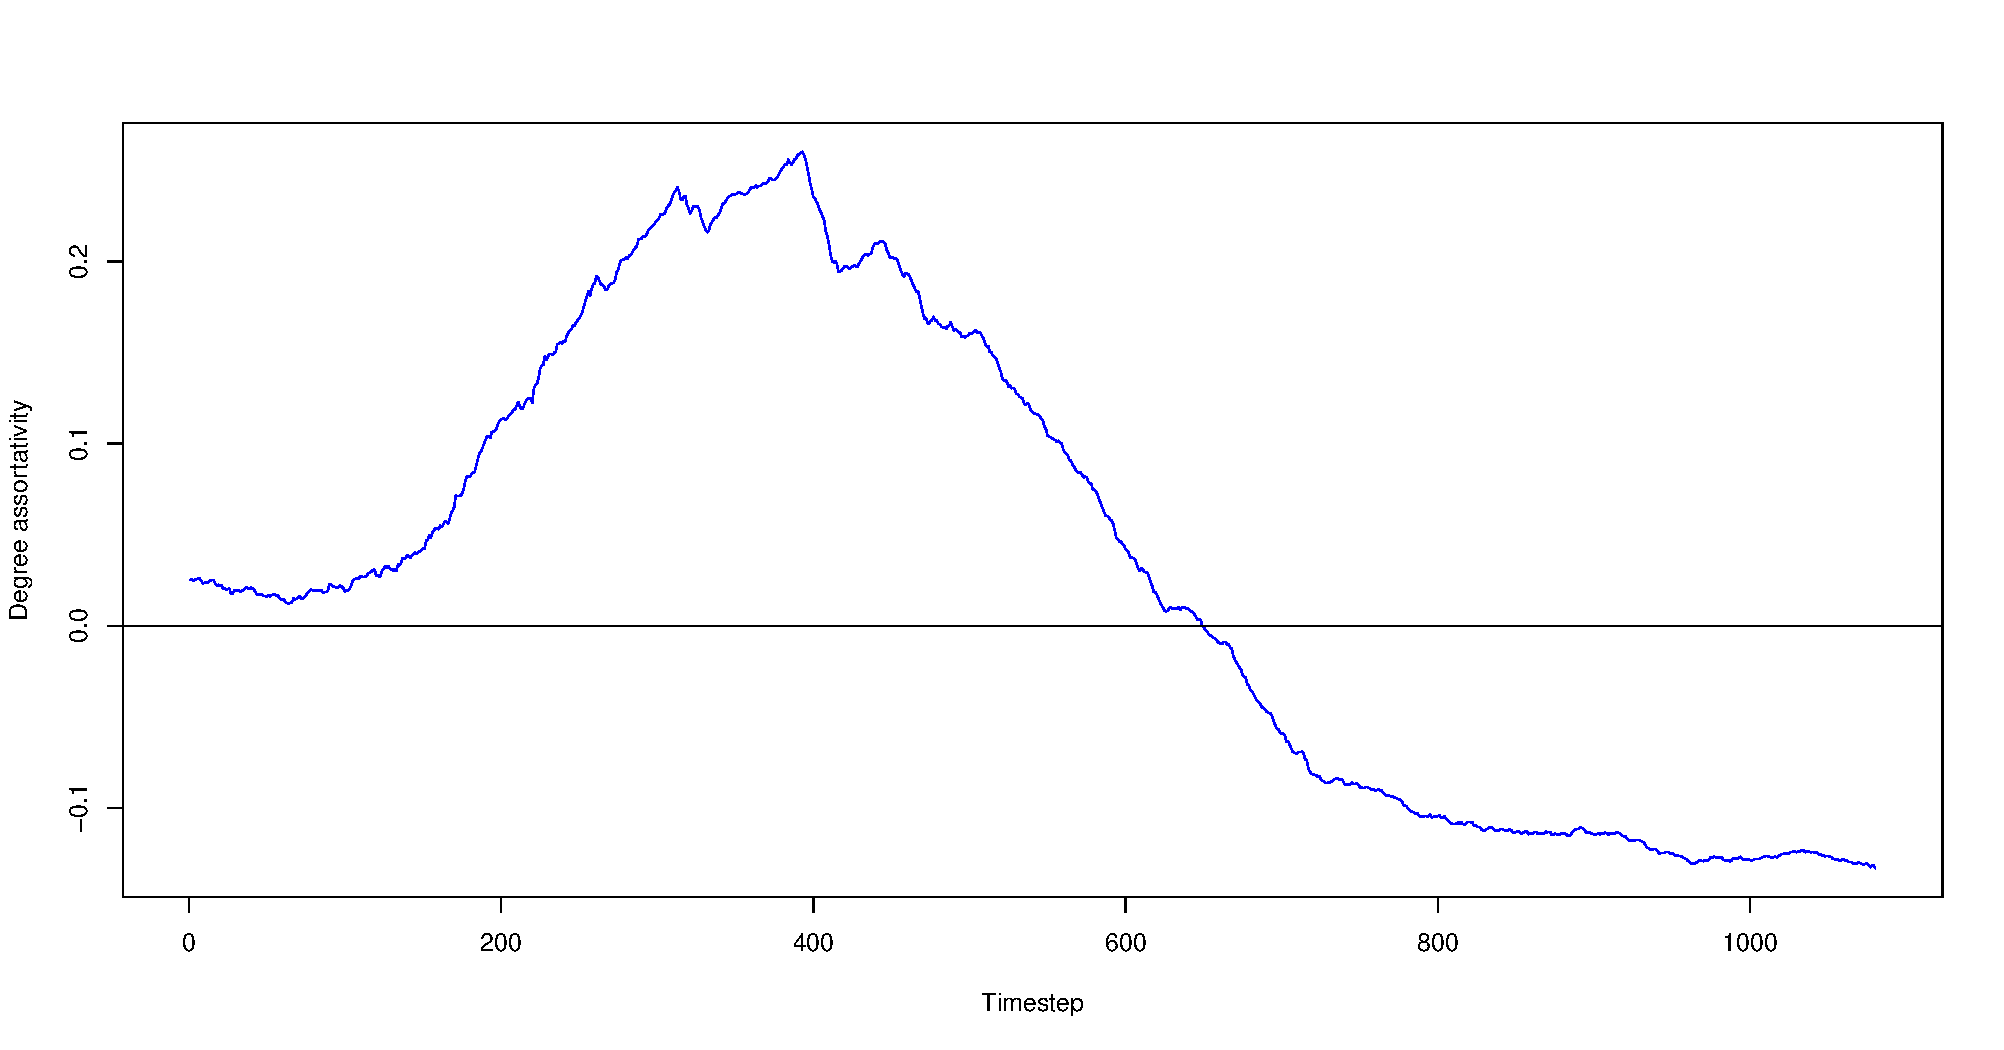
\includegraphics[width=81mm]{images/deg_assortativity_1000_rnd_1080_05_0.pdf} &   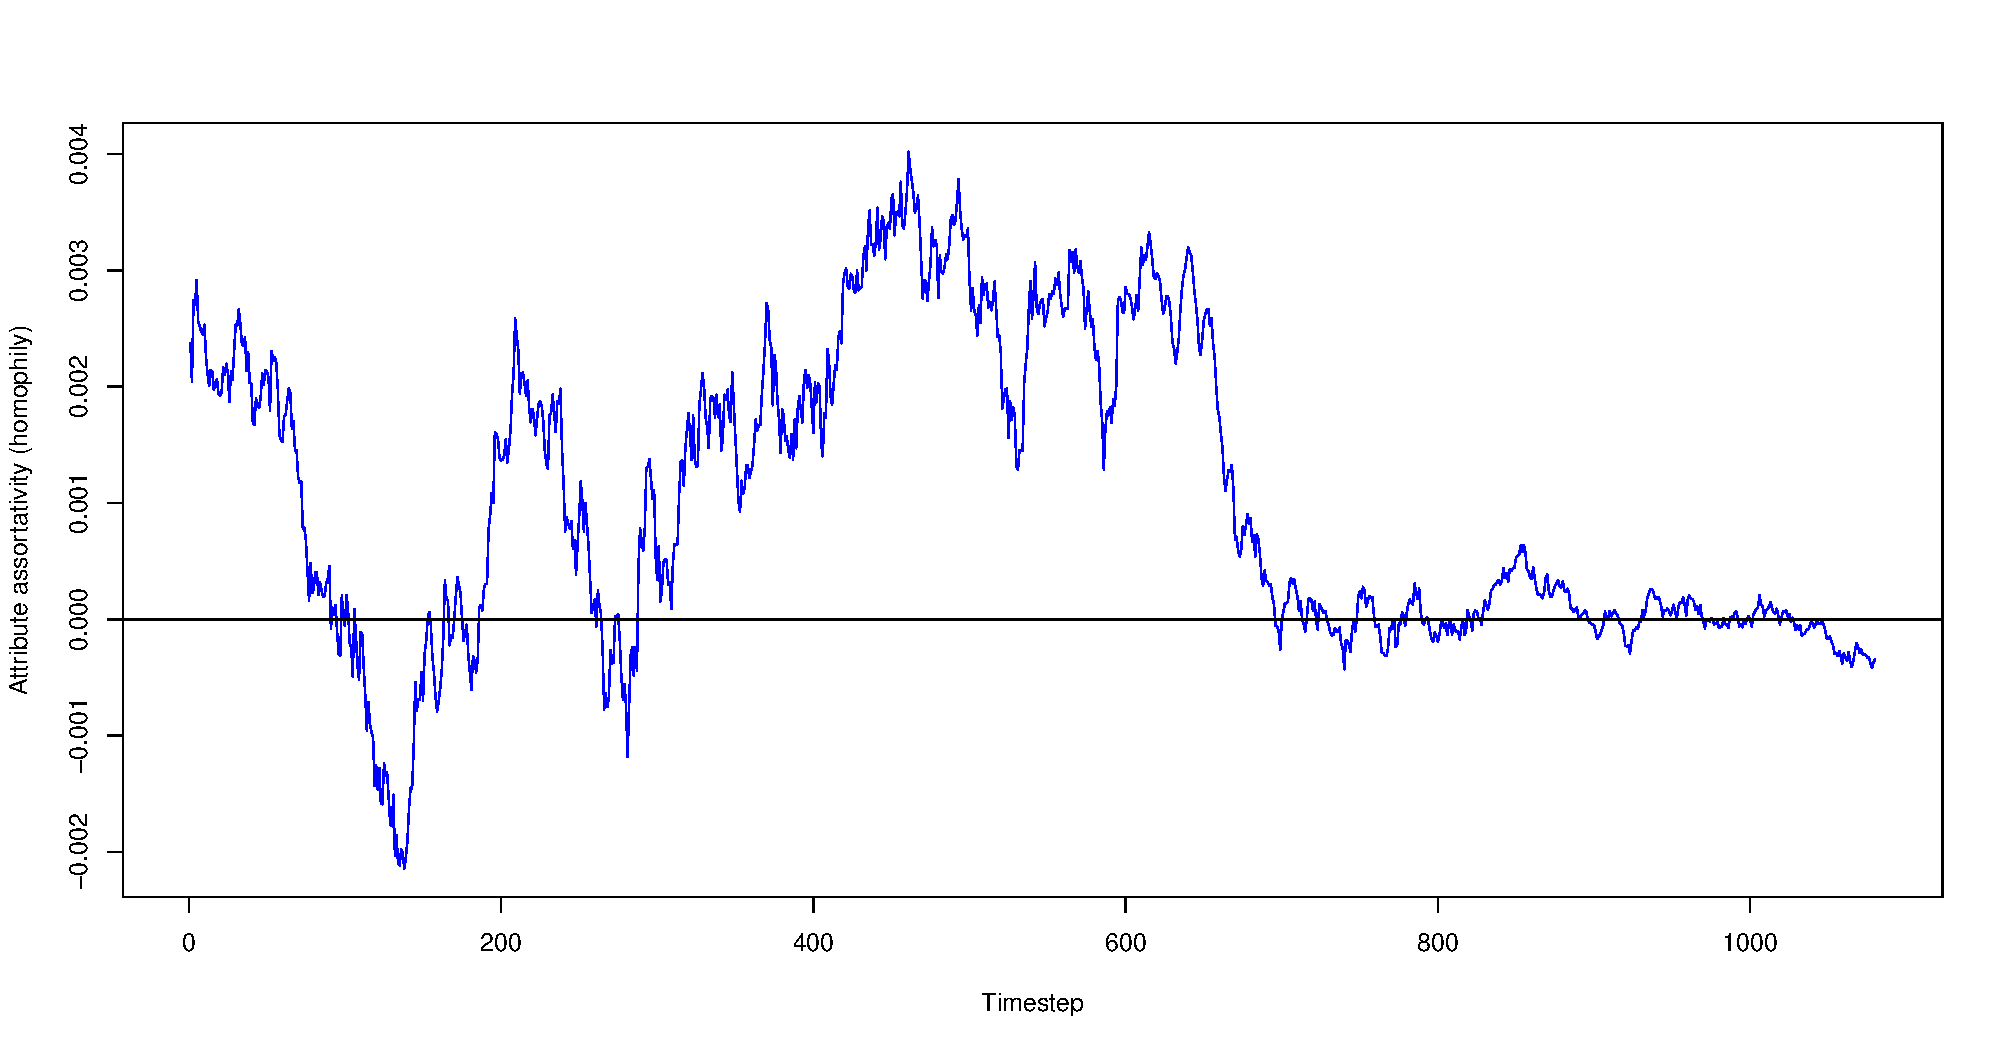
\includegraphics[width=81mm]{images/homophily_1000_rnd_1080_05_0.pdf} \\
c. Assortatività per grado & d. Assortatività per attributo \\[6pt]
\end{tabular}
\centering
\caption{Indici random network, densità 0.5\%}
\end{figure}
\\Il caso con densità di partenza pari a $0.5\%$ (figura 5) è piuttosto interessante, in quanto vi abbiamo osservato la crescita più rapida per quanto riguarda la densità: dallo $0.5\%$ iniziale, dopo una fase relativamente calma, cresce fino a superare il $6\%$ alla fine della simulazione. Questo si riflette sugli altri indici: ad esempio, il coefficiente di clustering, dopo un rapido incremento con una pendenza pari a quella assunta dalla densità, comicia a ridurre l'ascesa. Questo suggerisce che, man mano che la densità si fa importante, i collegamenti avvengo sempre di più all'interno di comunità già formate. Non solo: a partire dall'iterazione 984 la rete ha anche raggiunto lo stato di completa \textit{connessione}, ovvero la rete è diventata un'unica componente connessa; questo concorre all'affievolimento della crescita del coefficiente di clustering, in quanto favorisce l'instaurazione di archi intra-comunità. Nell'assortatività per grado si ritrova il fenomeno osservato nella prima run: l'indice cresce fino a raggiungere un picco, per poi calare fino alla fine delle iterazioni. Qui però il fenomeno è più rapido: il picco è più alto e viene raggiunto prima, mentre nella fase calante si verifica un livellamento improvviso, riscontrato anche nella misura di omofilia, dove l'assortatività per attributo si stabilizza sullo 0; questo comportamento può essere imputato al fatto che
\begin{figure}[t]
\begin{tabular}{cc}
  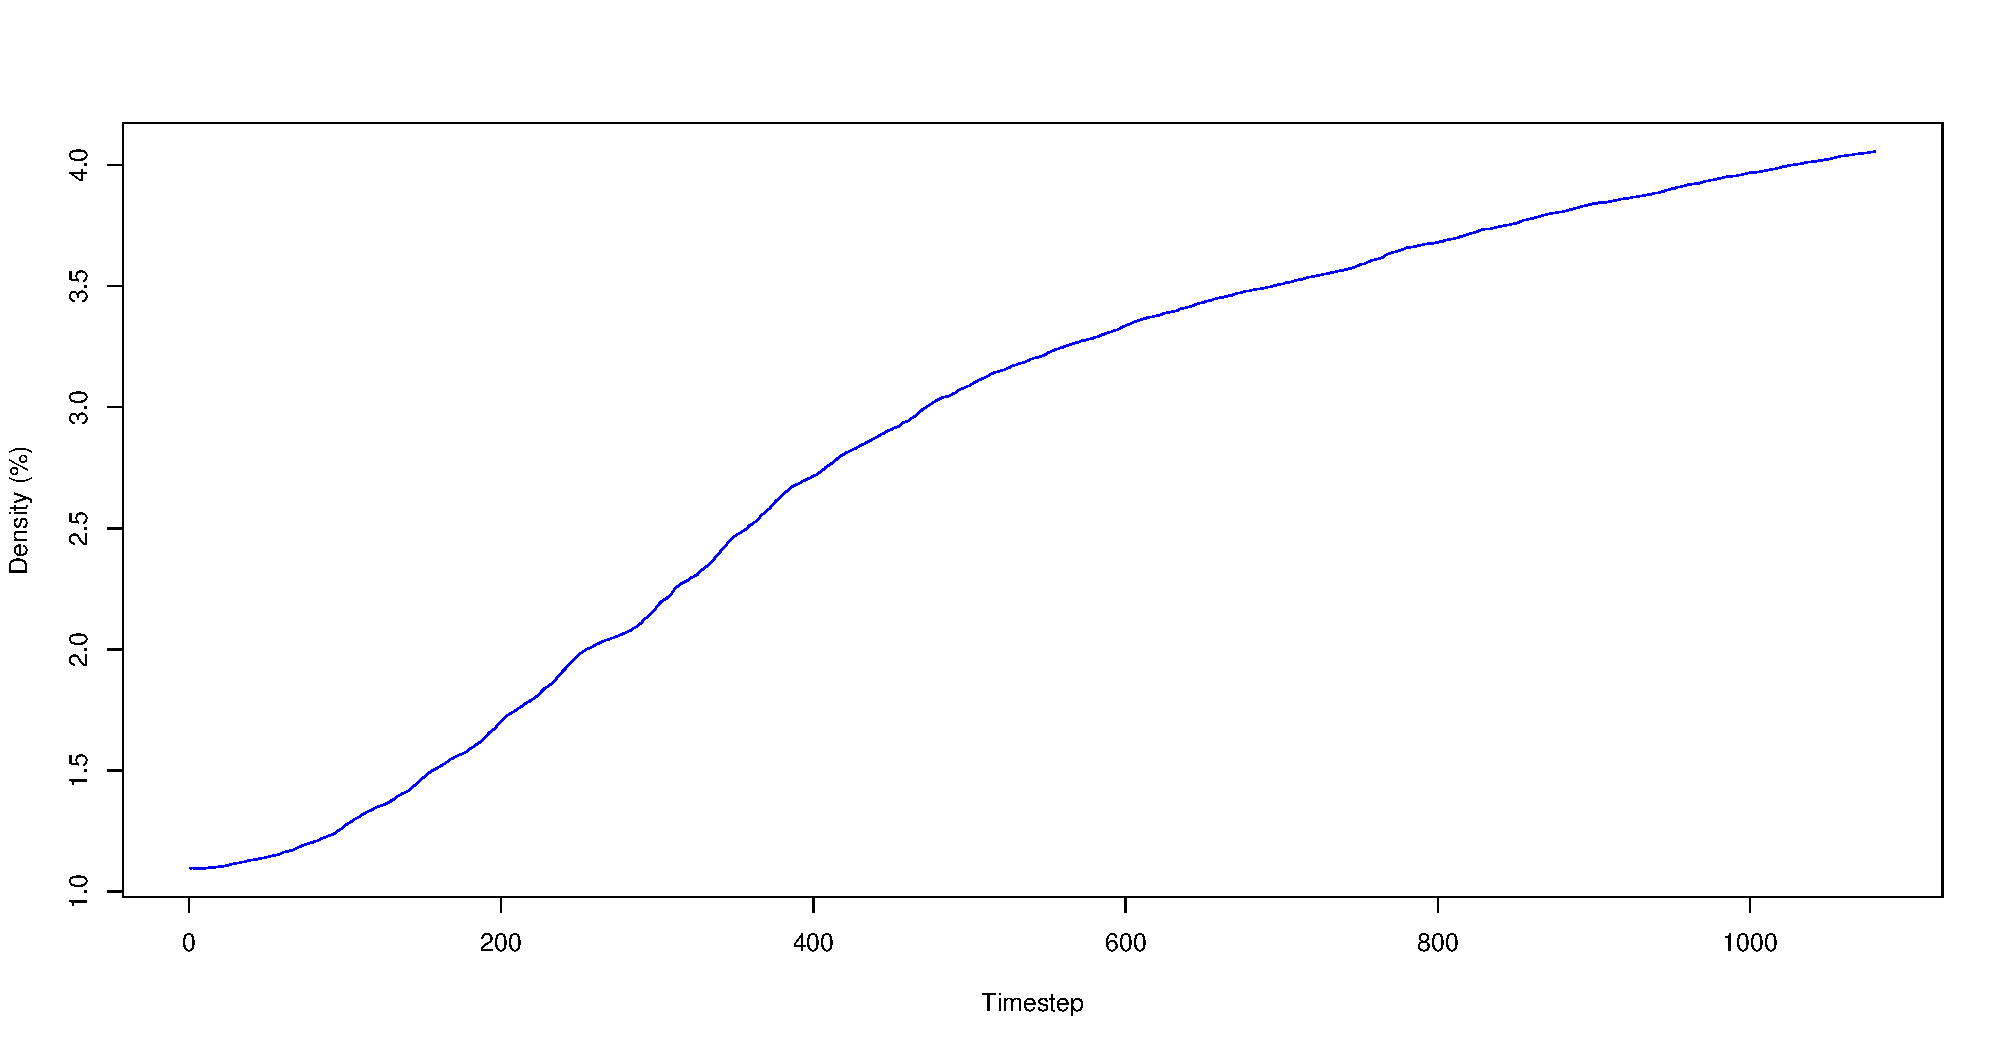
\includegraphics[width=81mm]{images/evolution_1000_rnd_1080_1_0.pdf} &   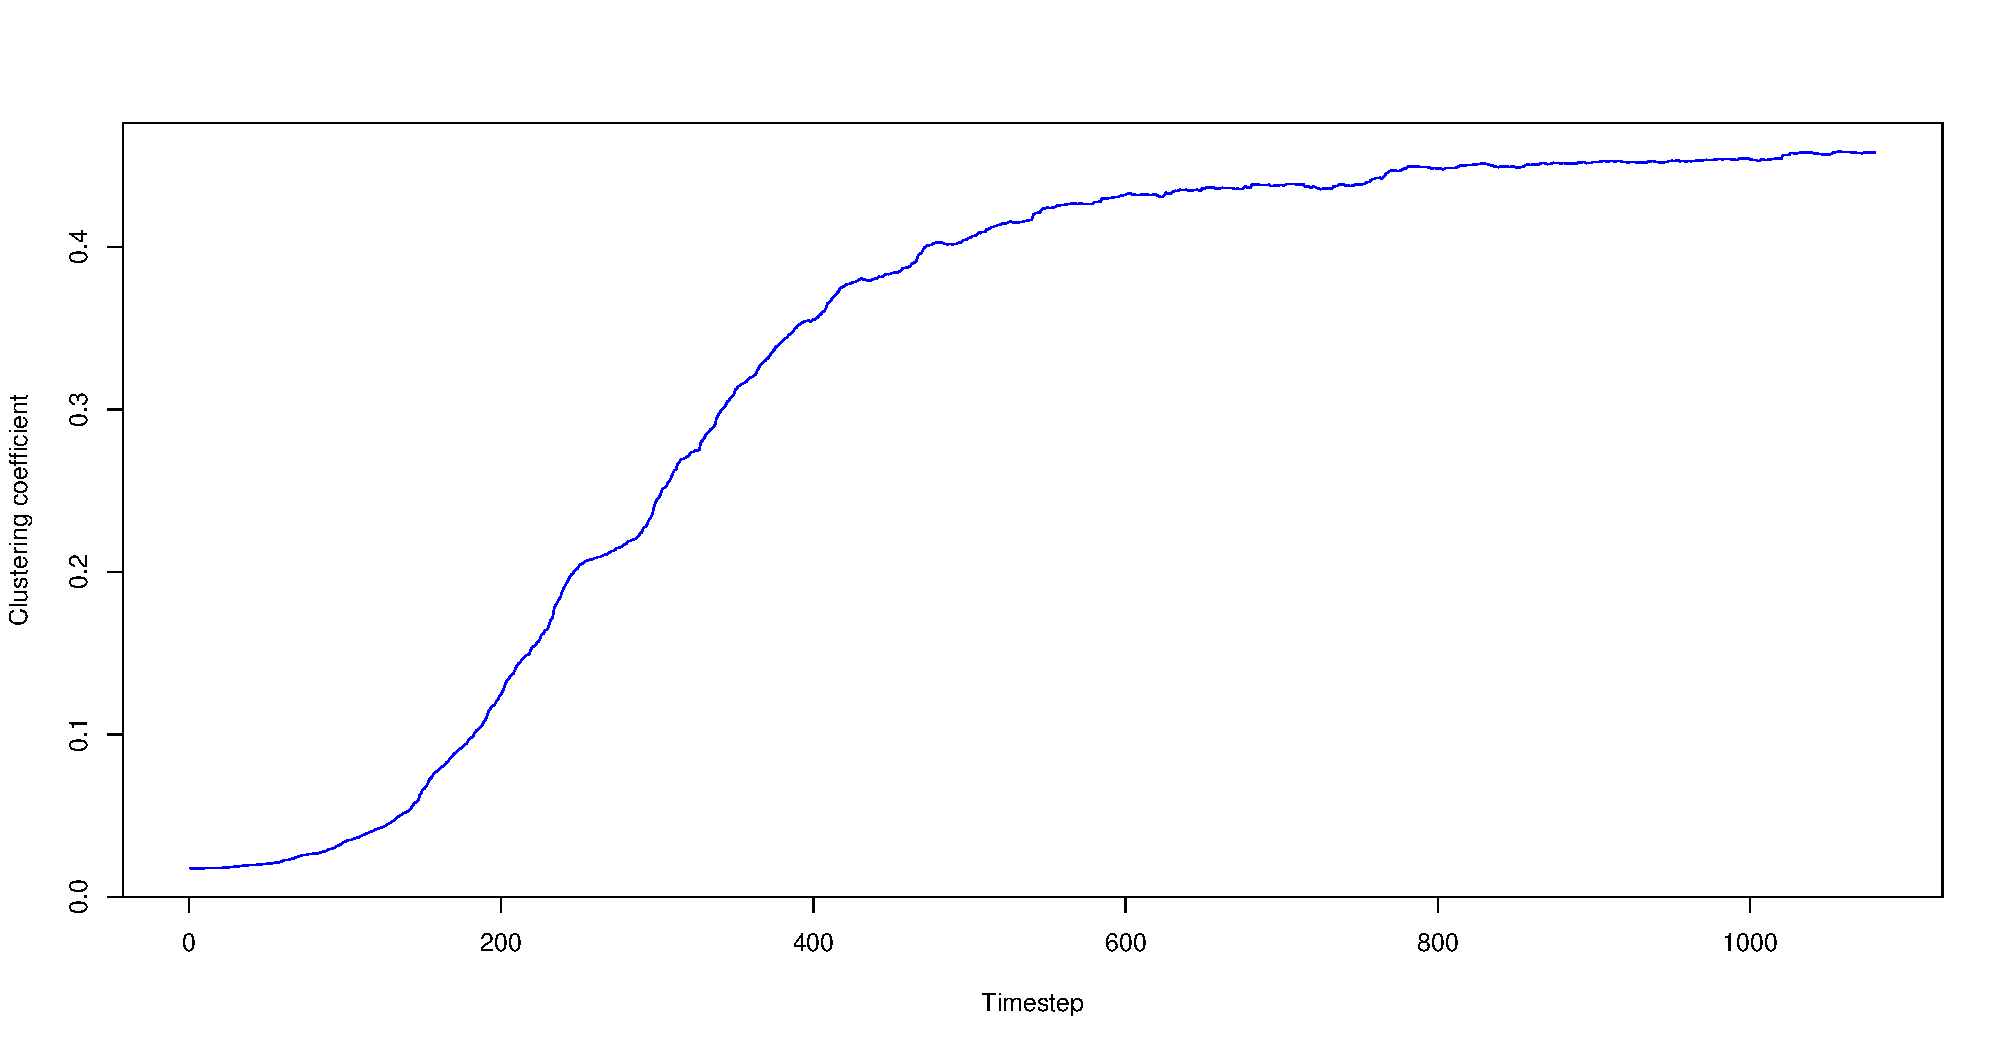
\includegraphics[width=81mm]{images/clustering_1000_rnd_1080_1_0.pdf} \\
a. Densità & b. Coefficiente di clustering \\[6pt]
 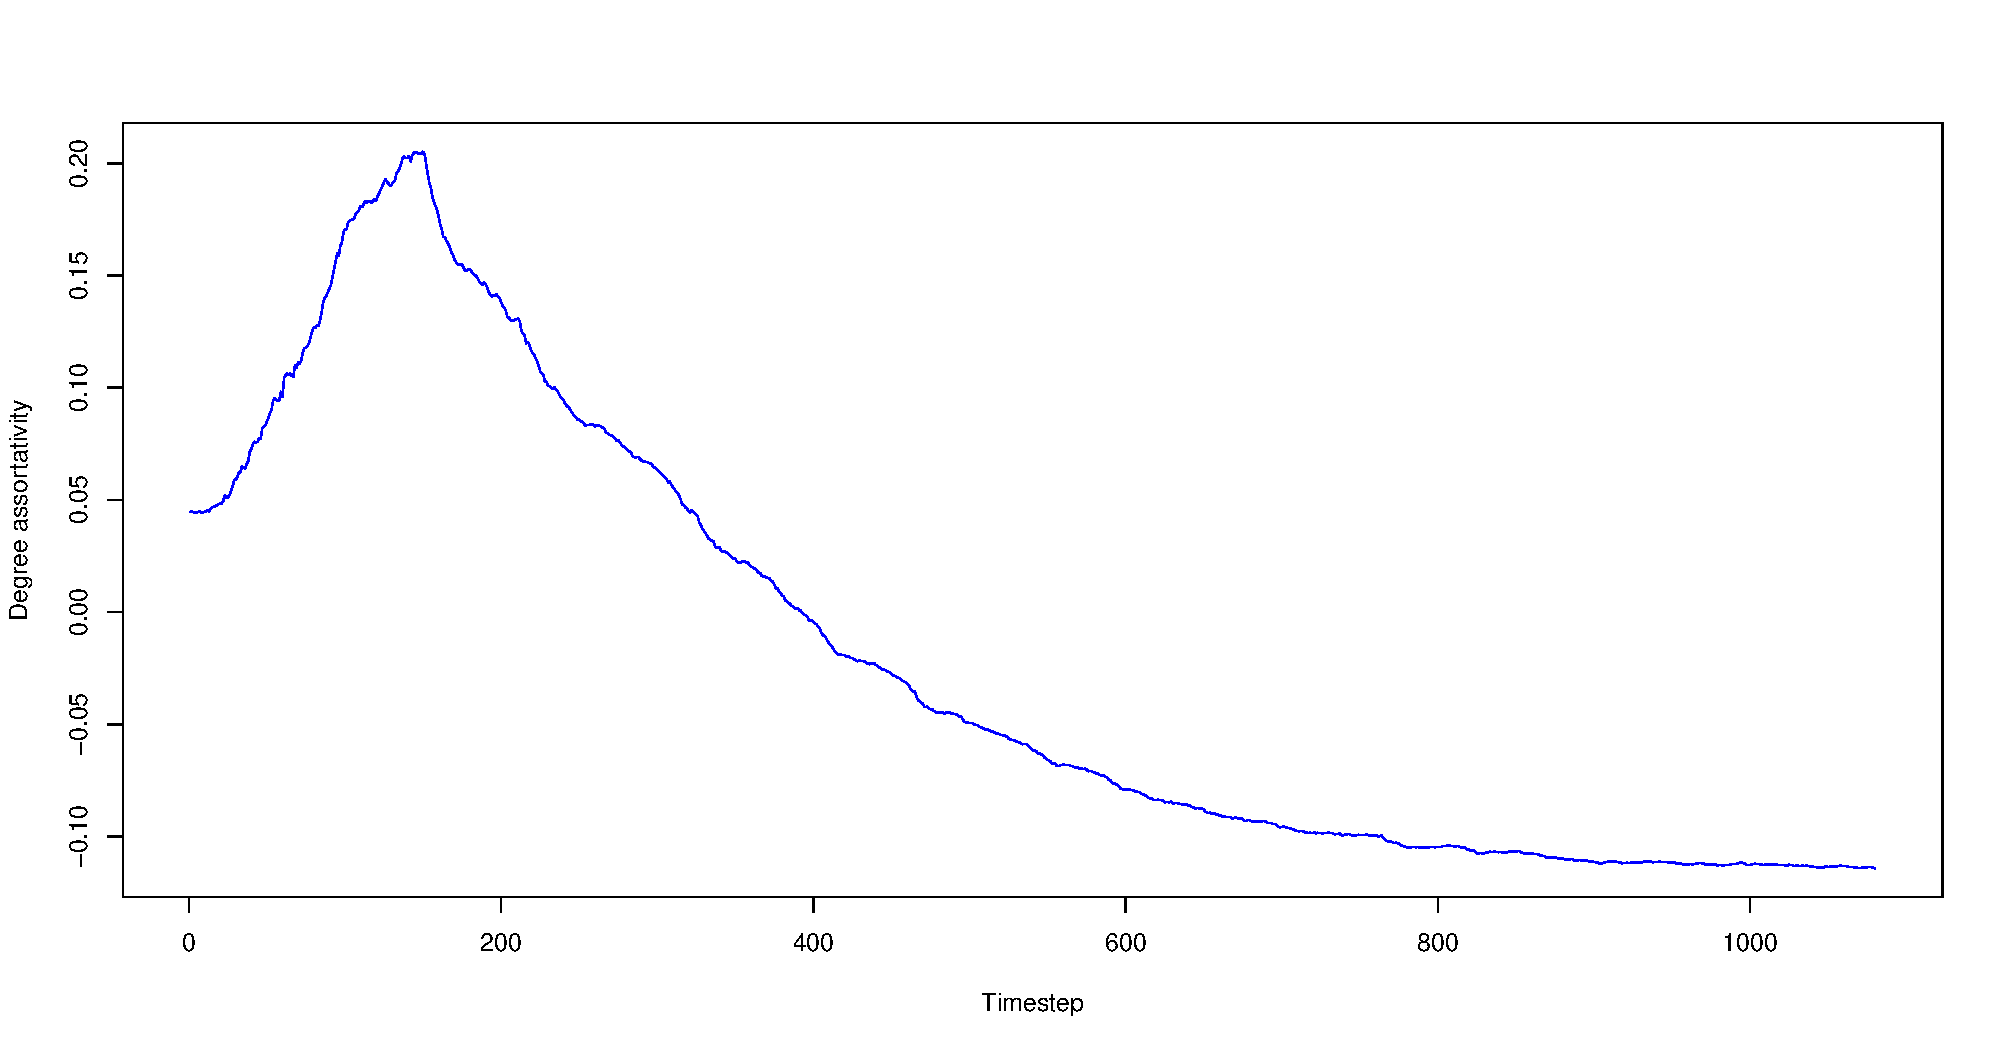
\includegraphics[width=81mm]{images/deg_assortativity_1000_rnd_1080_1_0.pdf} &   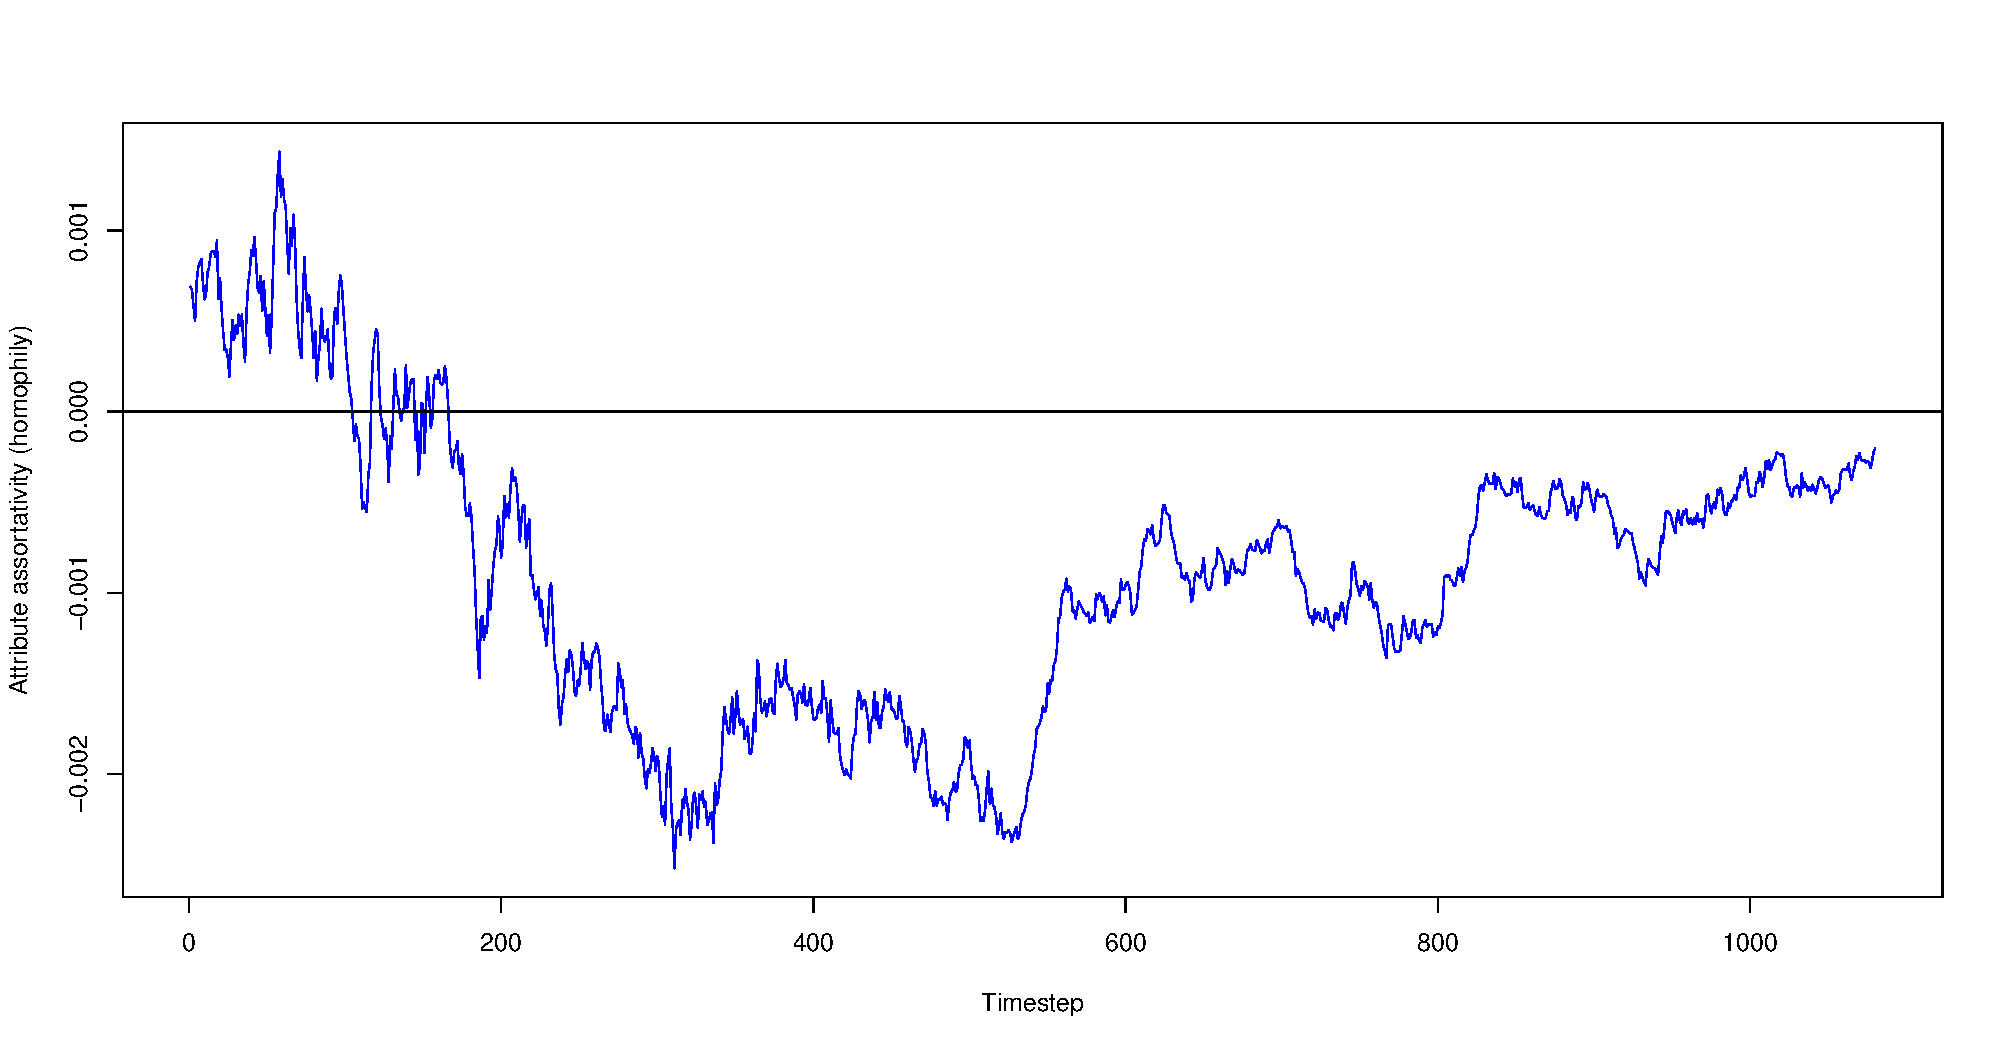
\includegraphics[width=81mm]{images/homophily_1000_rnd_1080_1_0.pdf} \\
c. Assortatività per grado & d. Assortatività per attributo \\[6pt]
\end{tabular}
\centering
\caption{Indici random network, densità 1.0\%}
\begin{tabular}{cc}
  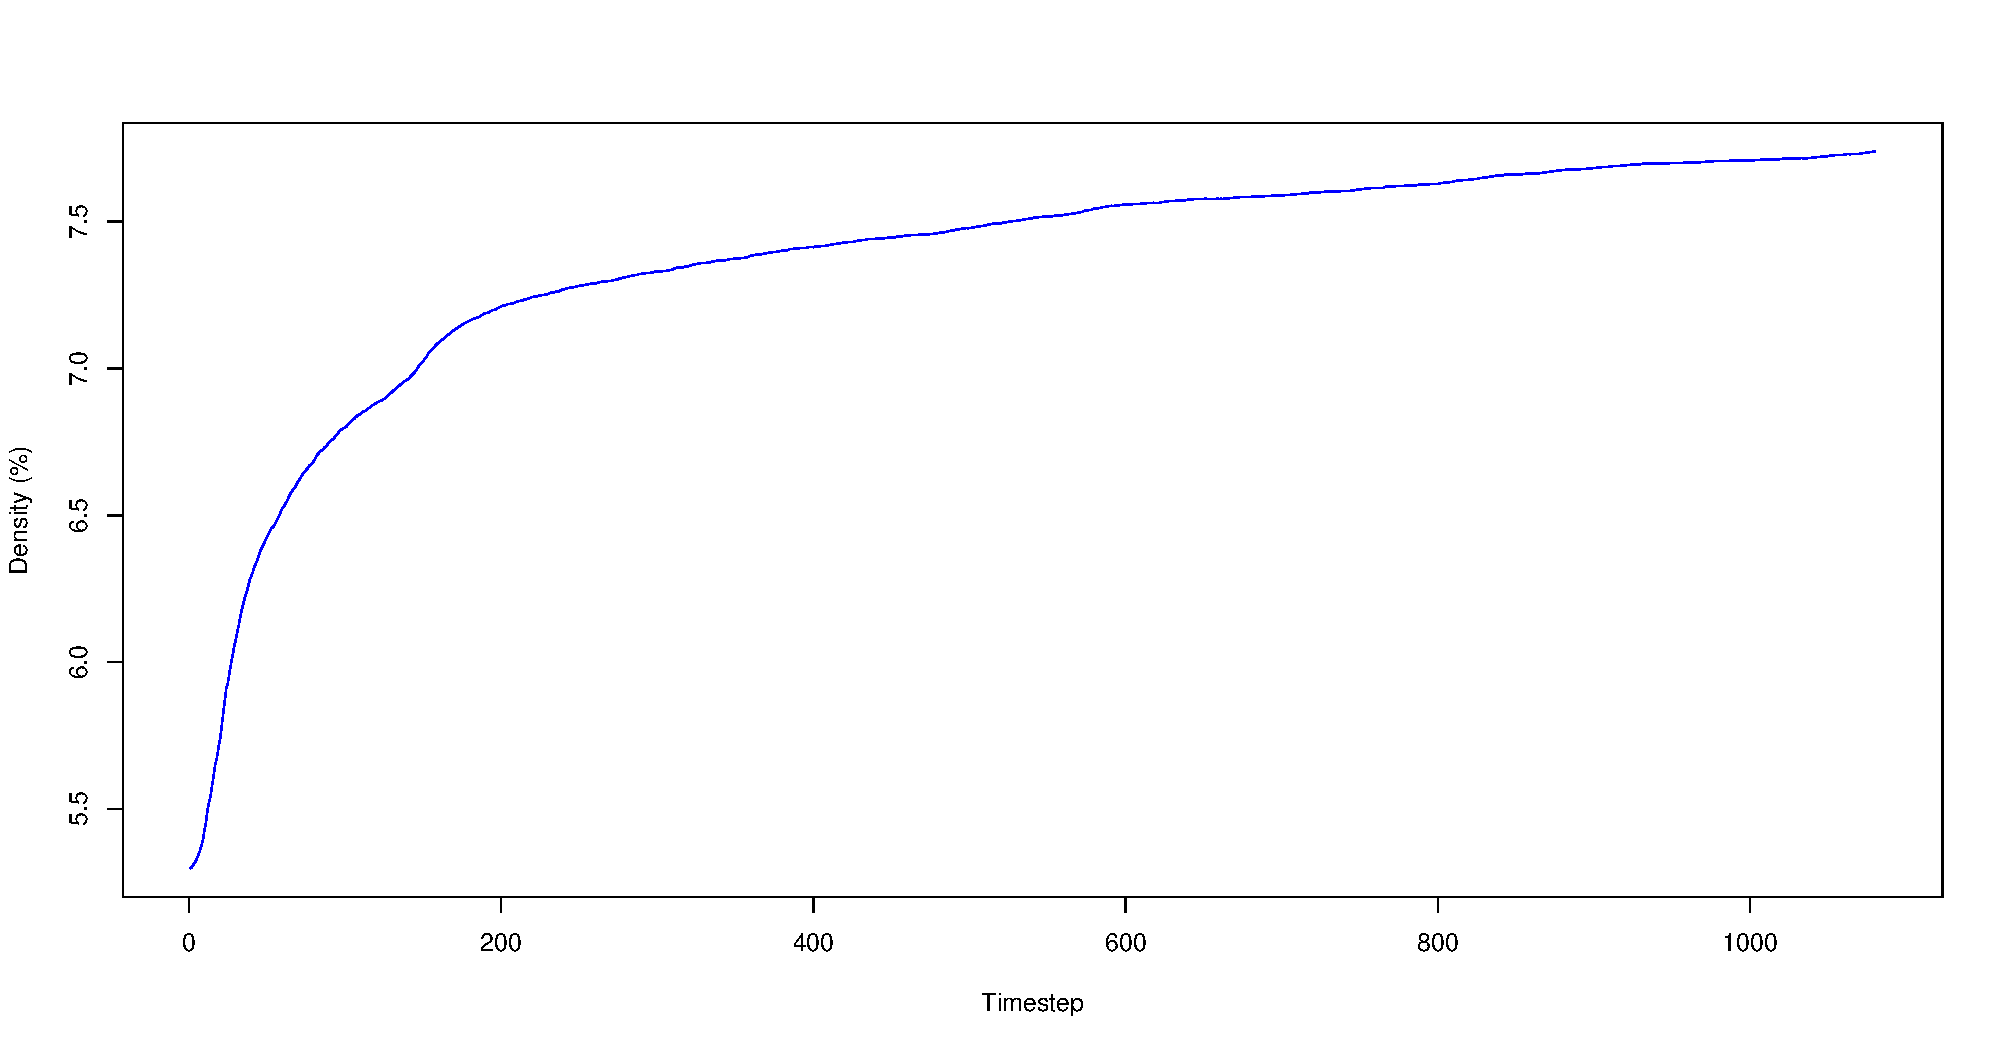
\includegraphics[width=81mm]{images/evolution_1000_rnd_1080_5_0.pdf} &   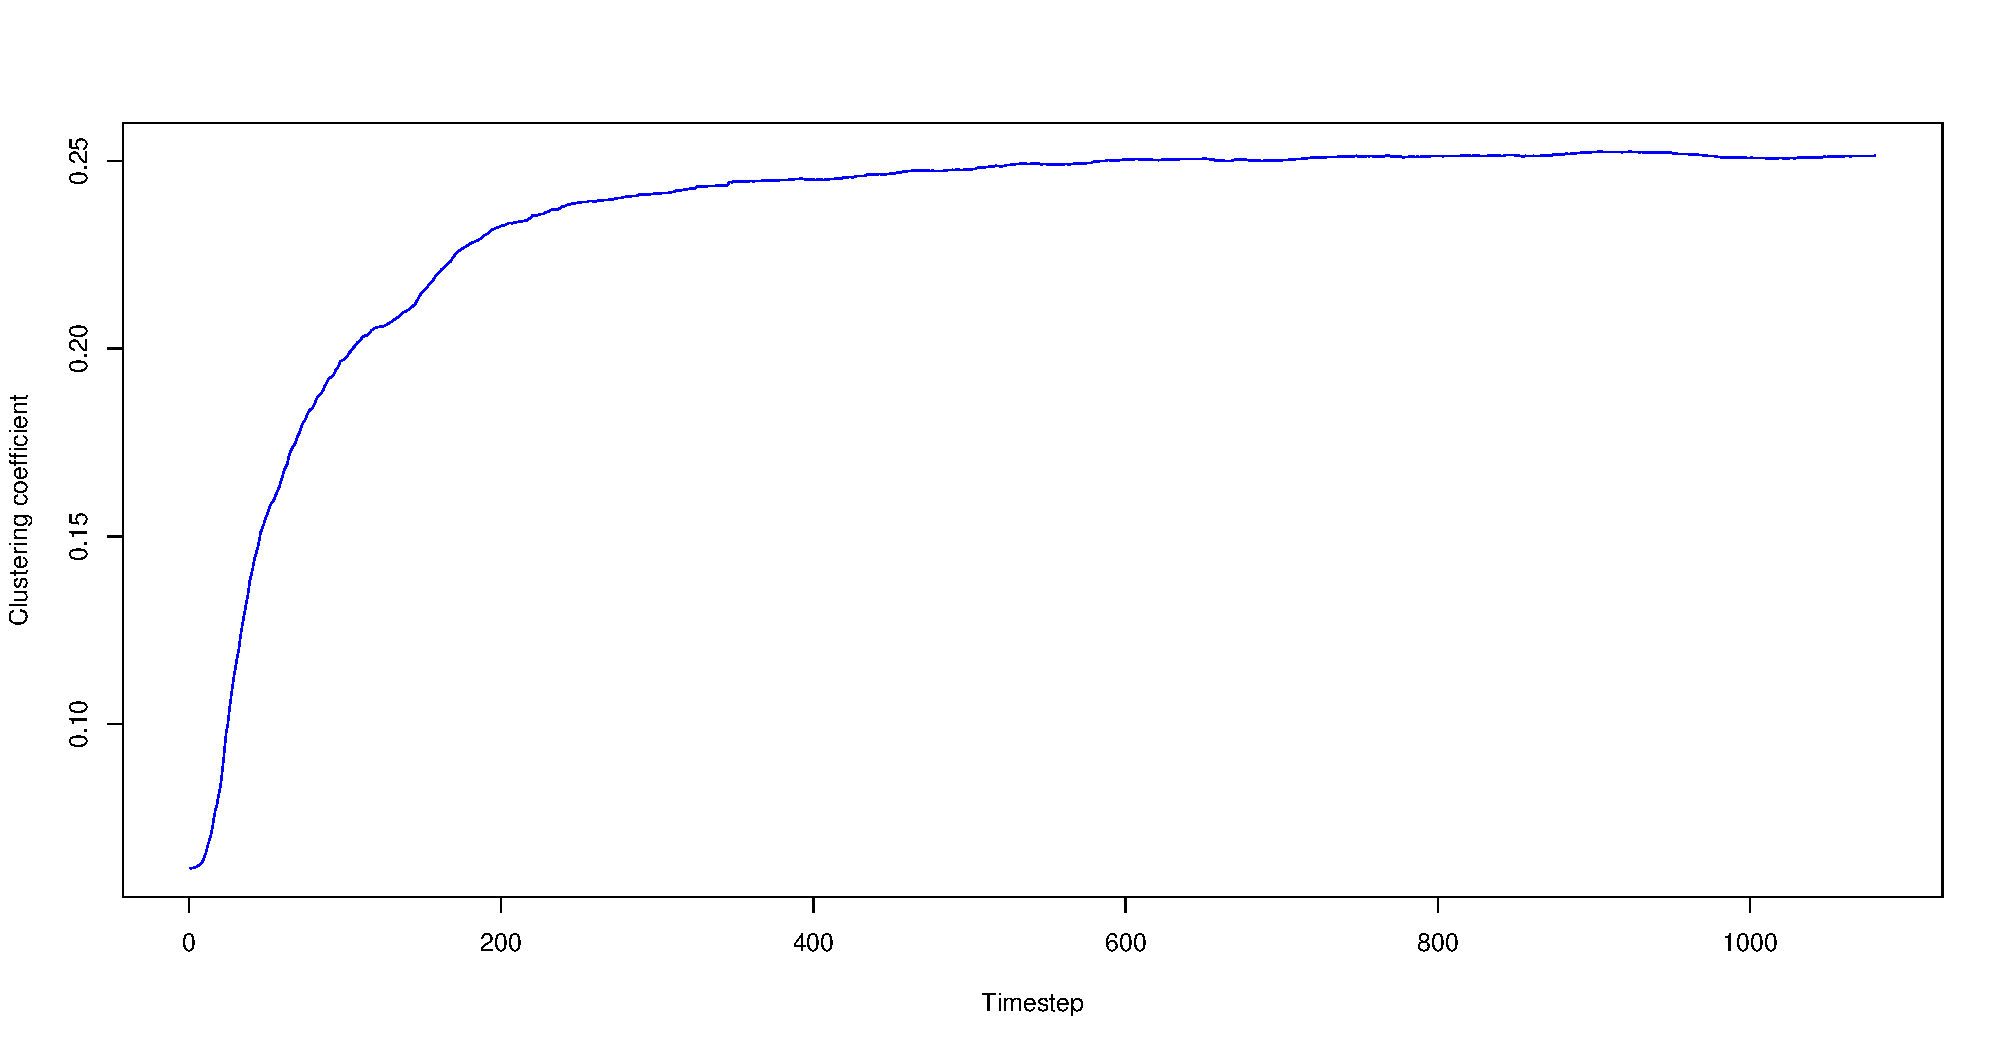
\includegraphics[width=81mm]{images/clustering_1000_rnd_1080_5_0.pdf} \\
a. Densità & b. Coefficiente di clustering \\[6pt]
 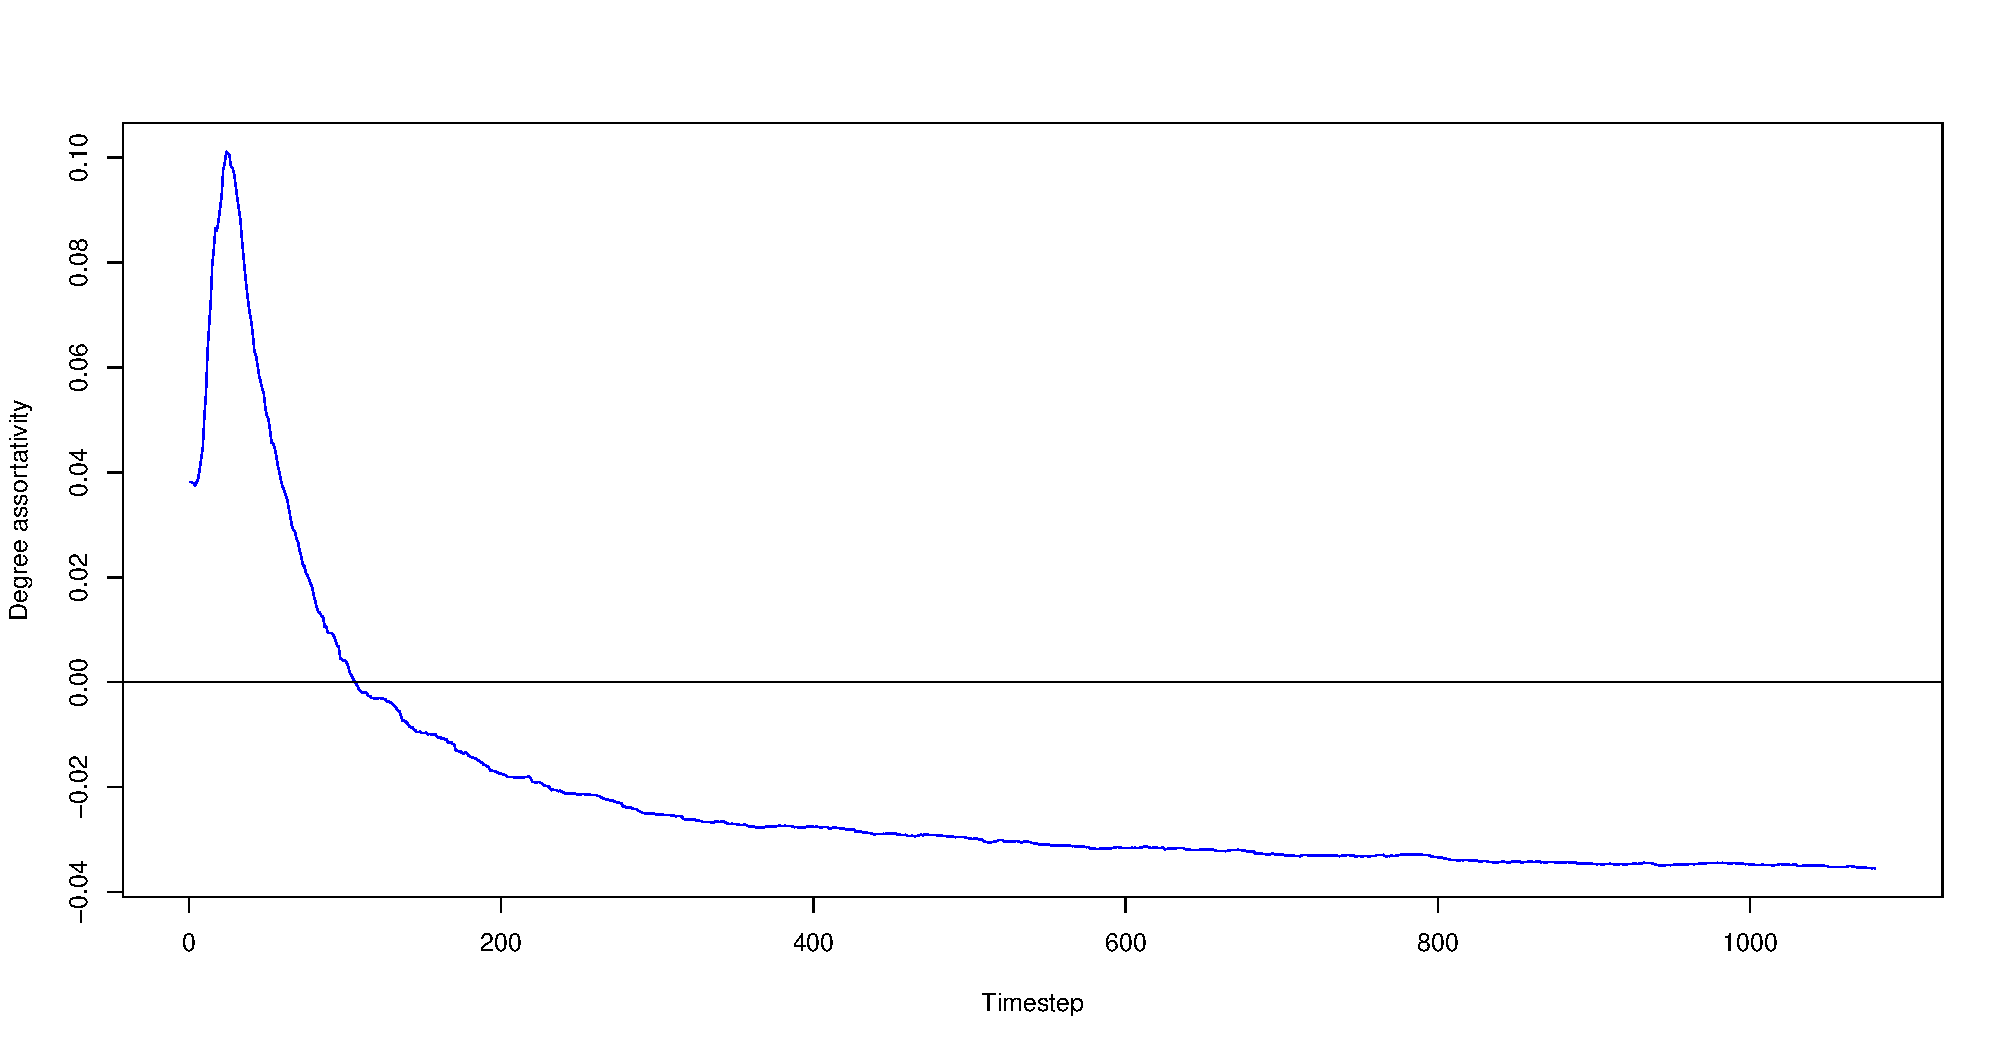
\includegraphics[width=81mm]{images/deg_assortativity_1000_rnd_1080_5_0.pdf} &   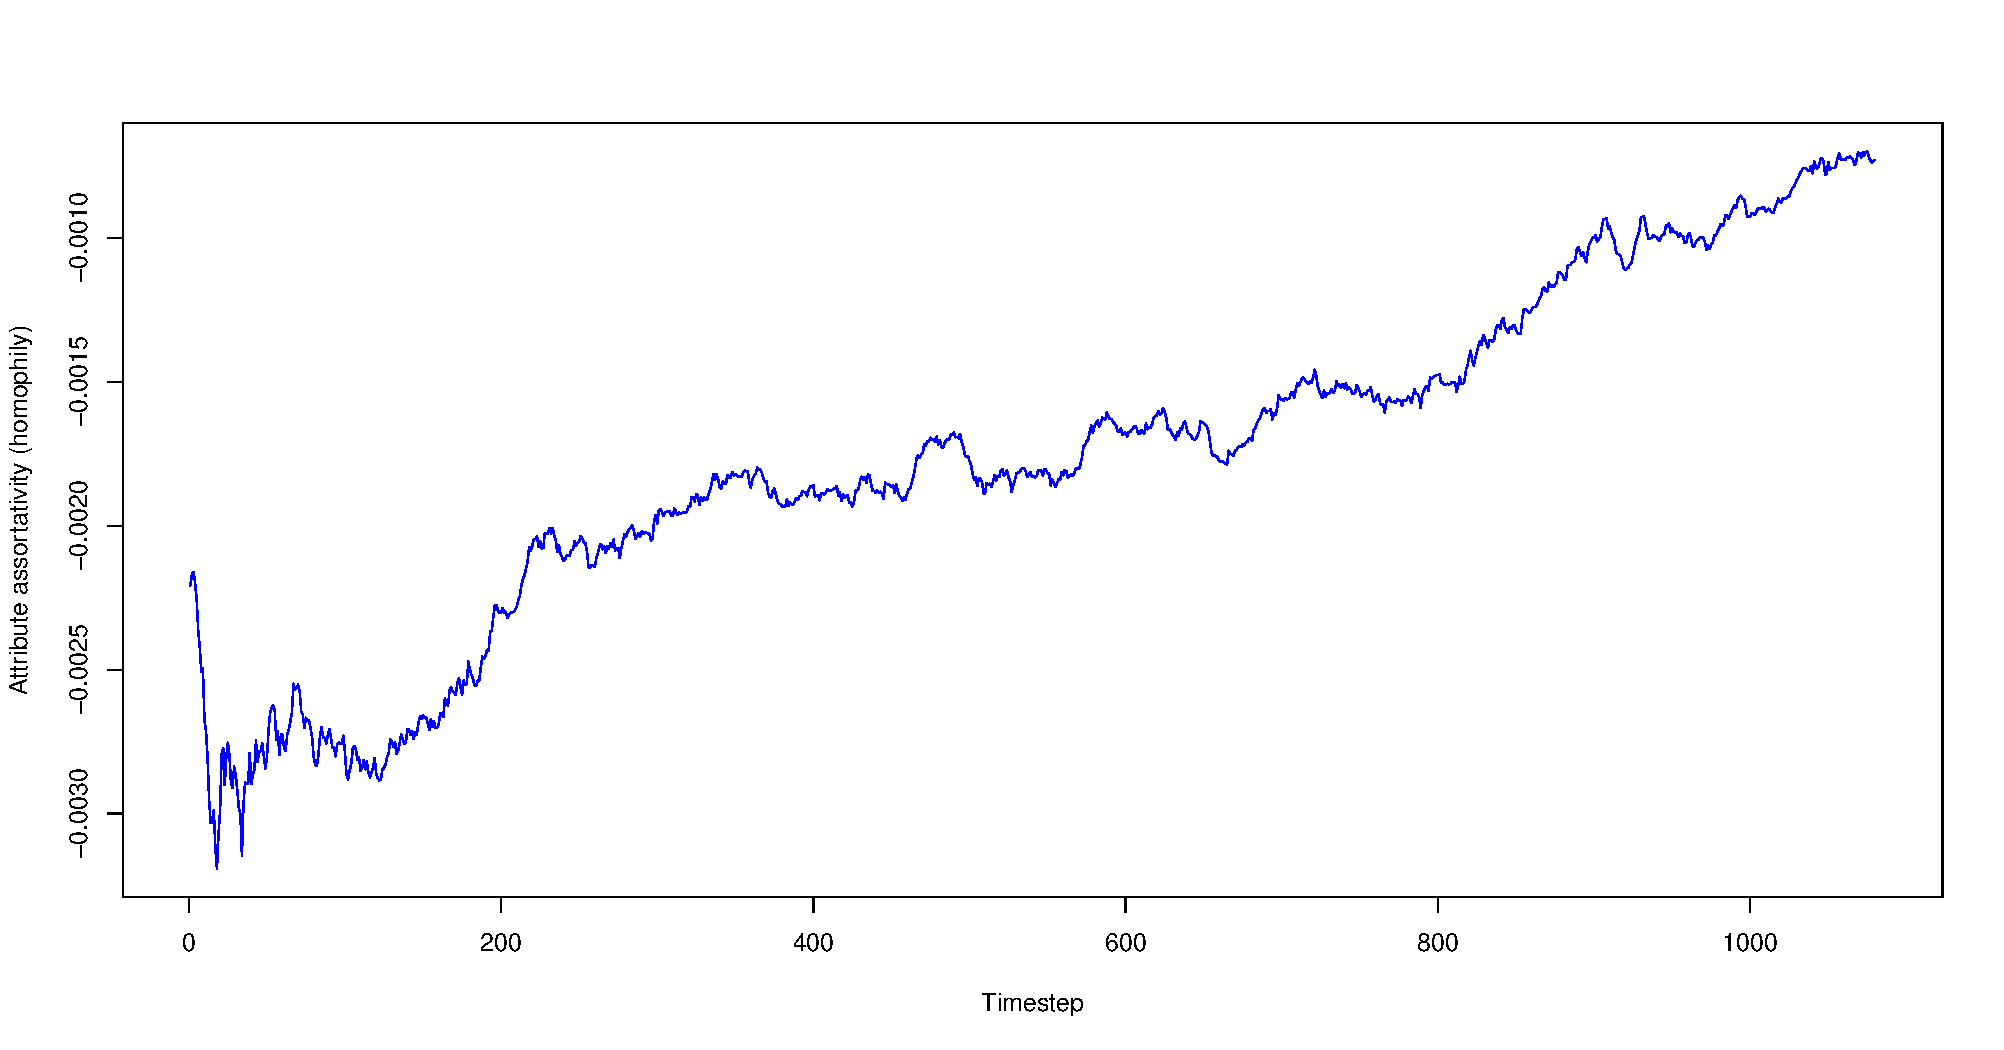
\includegraphics[width=81mm]{images/homophily_1000_rnd_1080_5_0.pdf} \\
c. Assortatività per grado & d. Assortatività per attributo \\[6pt]
\end{tabular}
\centering
\caption{Indici random network, densità 5.0\%}
\end{figure}

\begin{figure}[b]
\begin{tabular}{cc}
  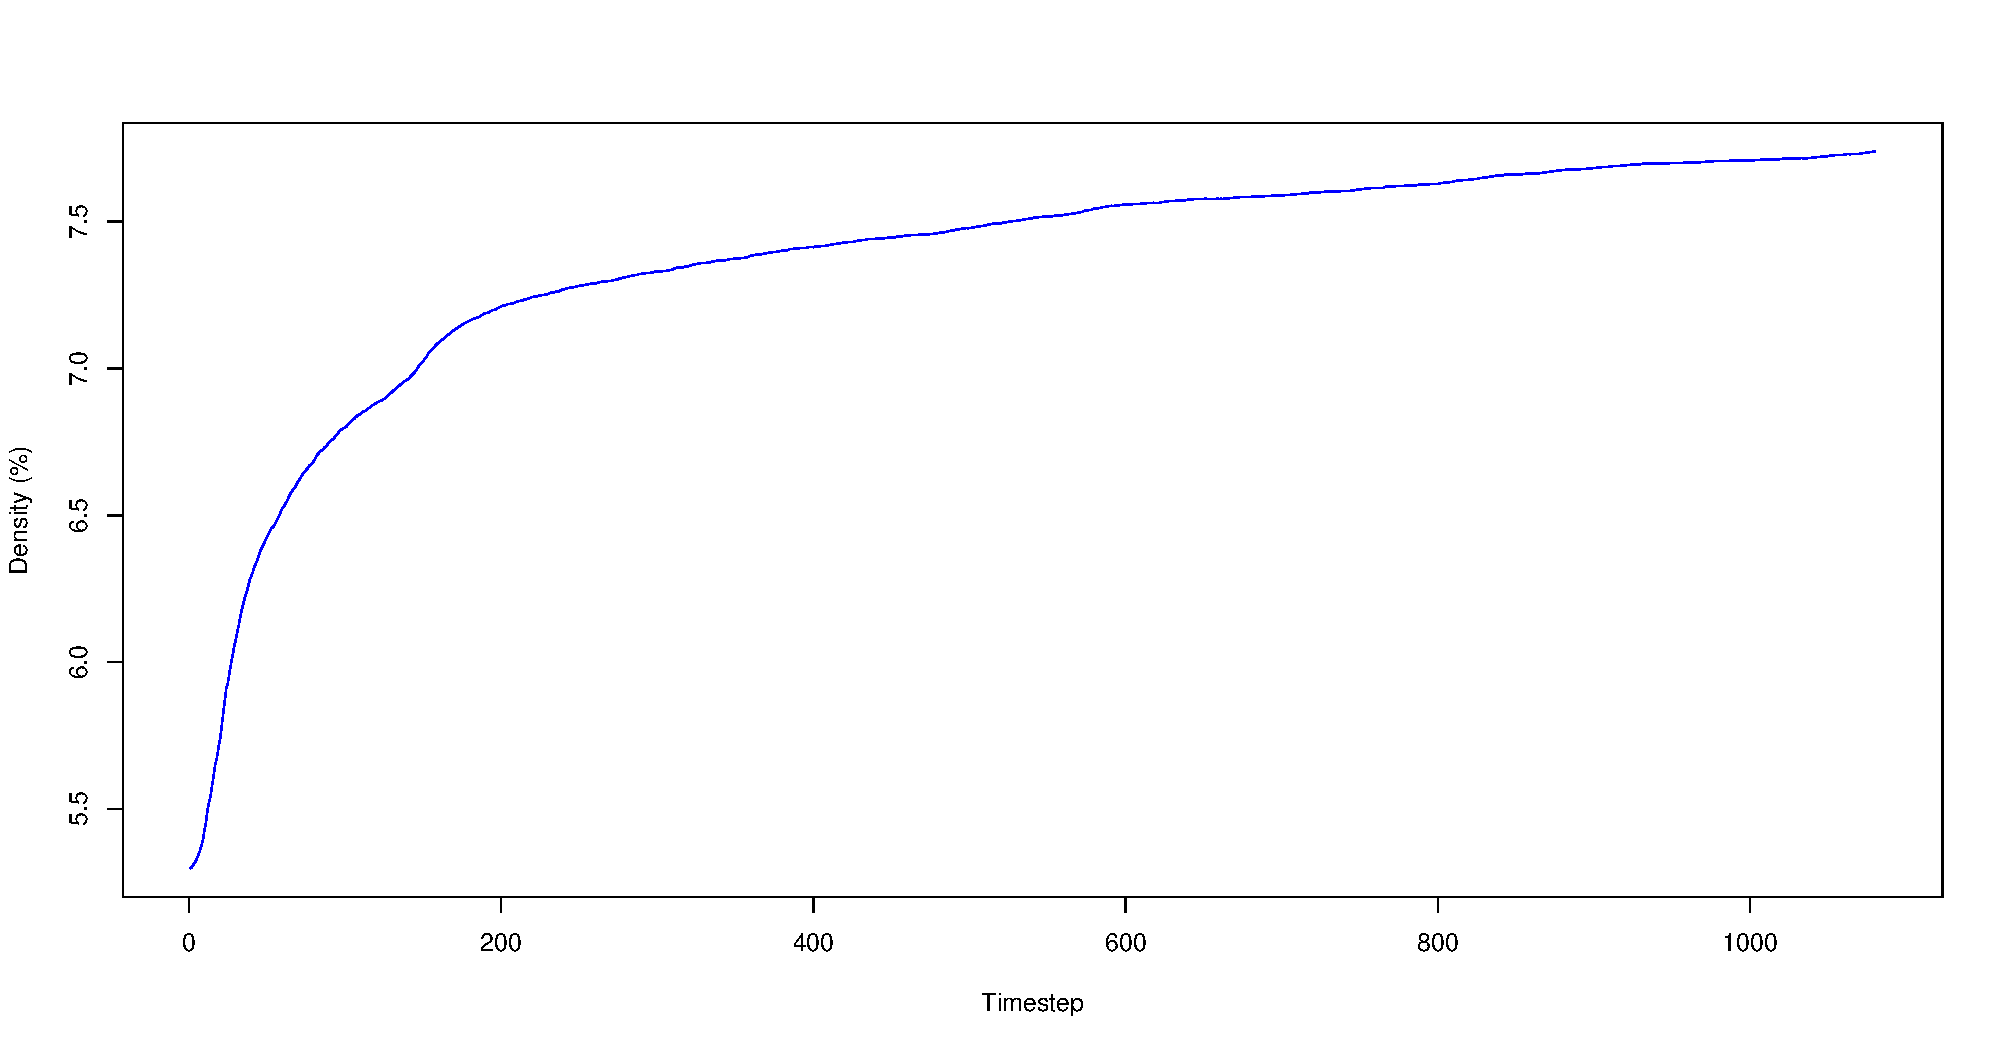
\includegraphics[width=81mm]{images/evolution_1000_rnd_1080_5_0.pdf} &   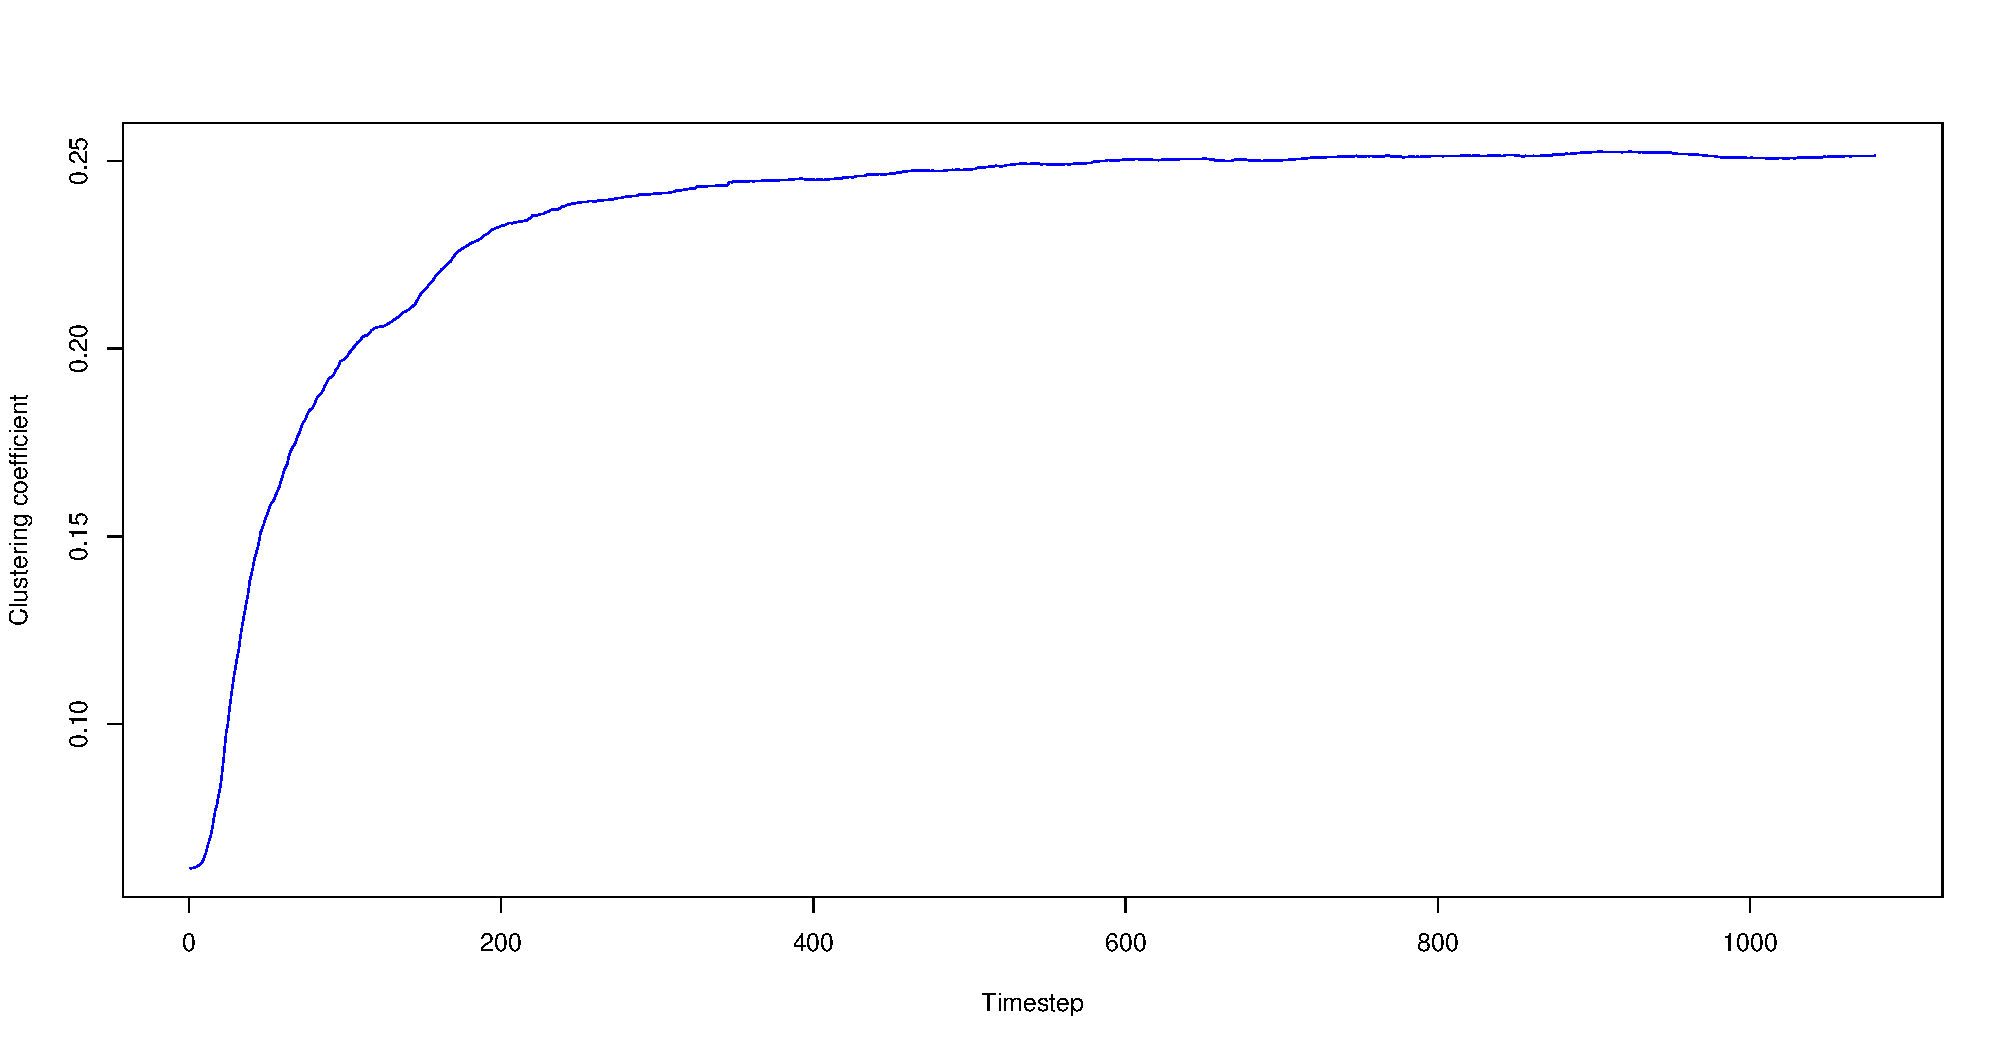
\includegraphics[width=81mm]{images/clustering_1000_rnd_1080_5_0.pdf} \\
a. Densità & b. Coefficiente di clustering \\[6pt]
 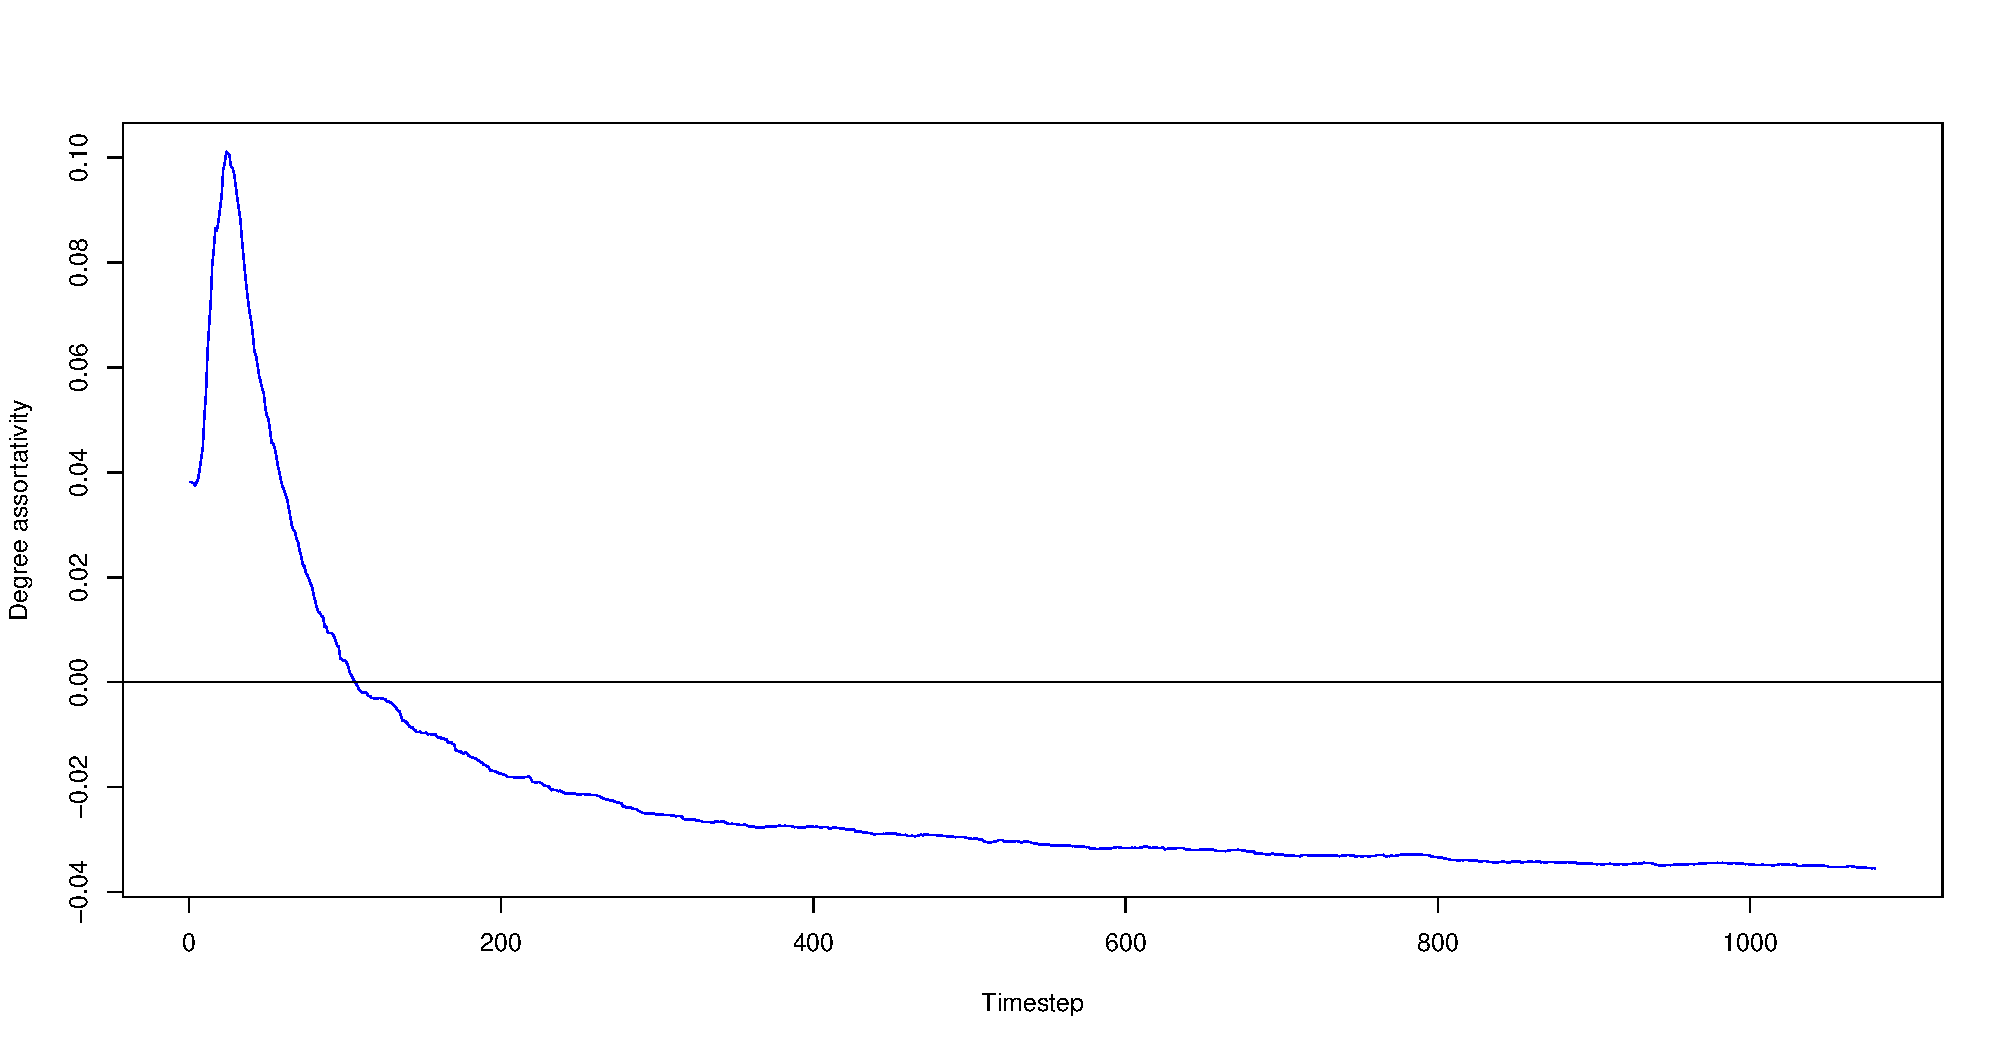
\includegraphics[width=81mm]{images/deg_assortativity_1000_rnd_1080_5_0.pdf} &   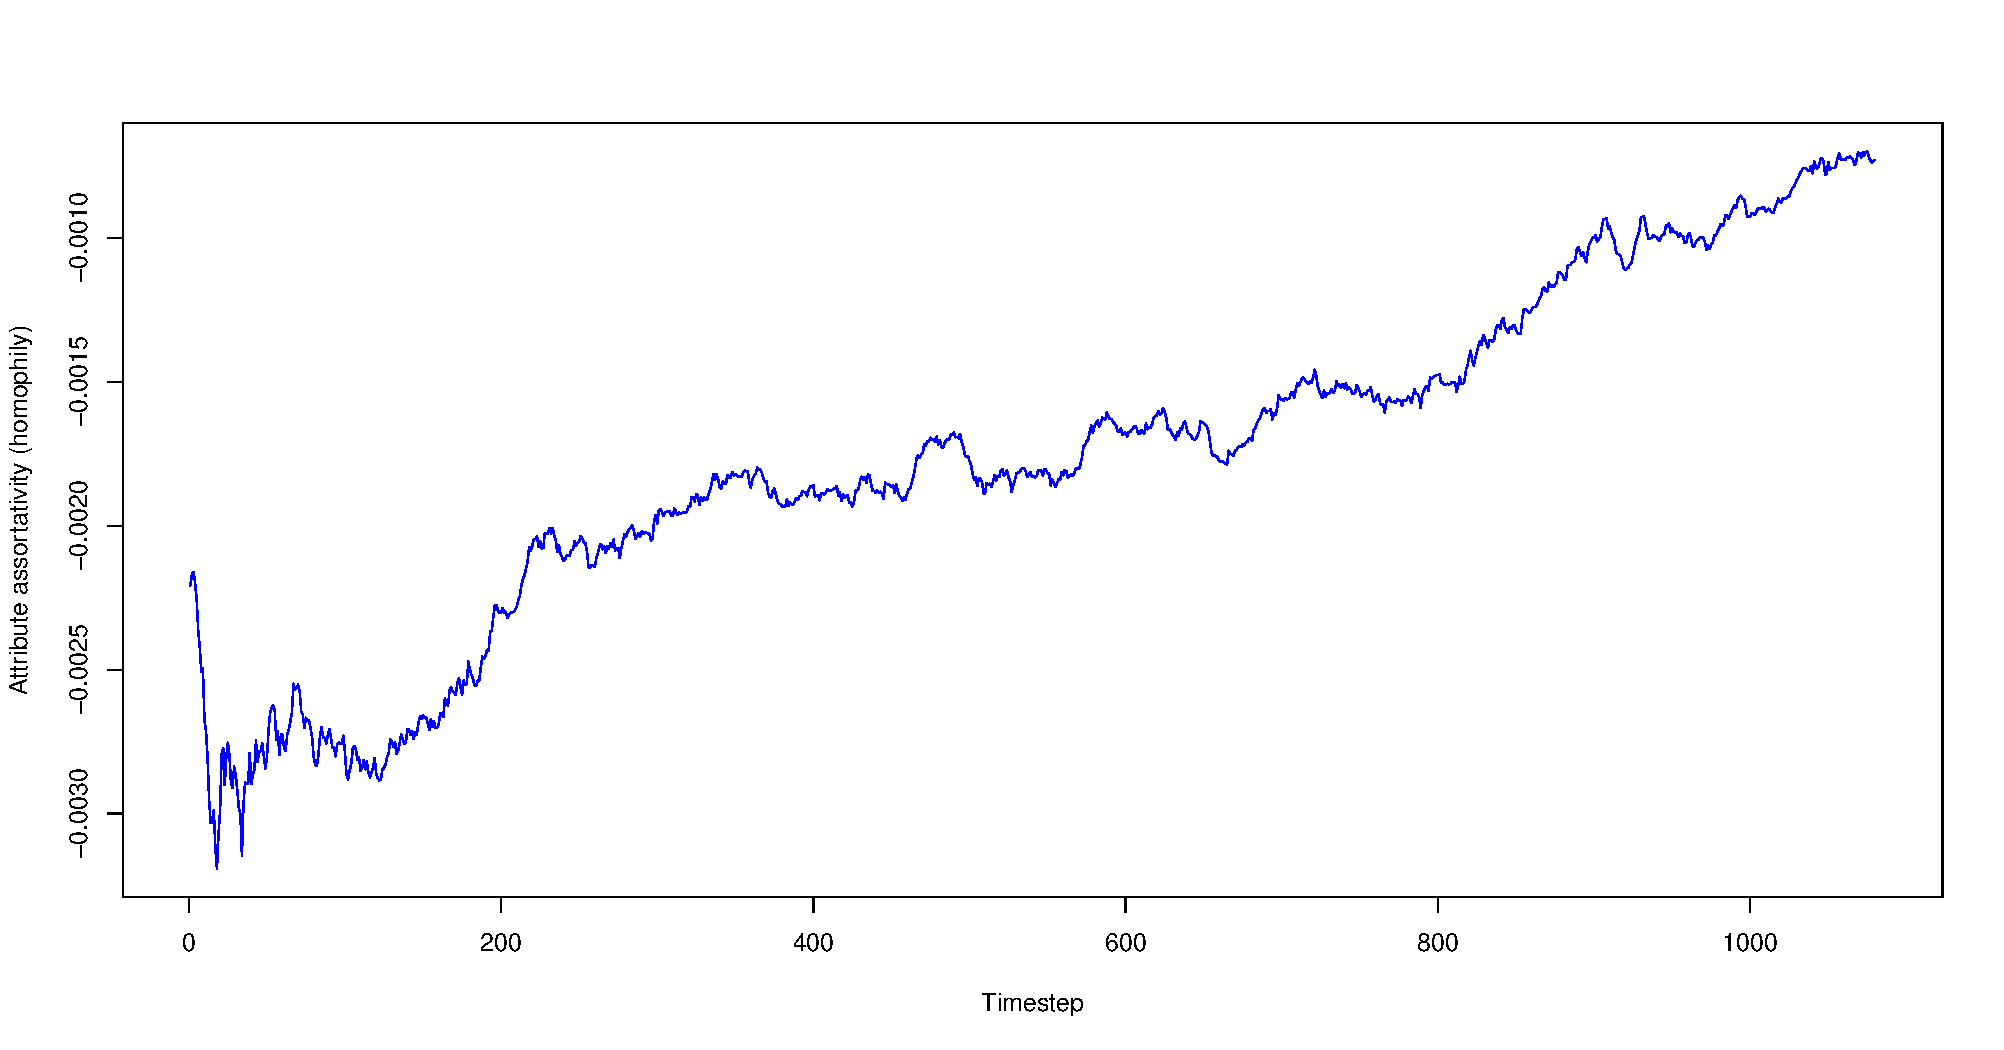
\includegraphics[width=81mm]{images/homophily_1000_rnd_1080_5_0.pdf} \\
c. Assortatività per grado & d. Assortatività per attributo \\[6pt]
\end{tabular}
\centering
\caption{Indici random network, densità 5.0\%}
\end{figure}

\subsection{Fase 2}
\section{Conclusione}
\label{sec:end}
\section{Sviluppi futuri}
\label{sec:future}


\begin{thebibliography}{9}
\bibitem{facebook}
  Welch, Chris (2017). "Facebook crosses 2 billion monthly users". \textit{The Verge. Vox Media.} Retrieved June 27, 2017.
  
\bibitem{twitter}
  Bulman, May (2016). ``Donald Trump's 'celebrity-style' tweets helped him win US presidential election, says data scientist".
\textit{The Independent} Retrieved November 28, 2016.

\bibitem{youtube}
   Sorkin, Andrew Ross \& Peters, Jeremy, W. (2006). ``Google to Acquire YouTube for \$1.65 Billion". \textit{The New York Times.} Retrieved October 9, 2006.

\bibitem{linkedin}
   Greene, Jay (2016). ``Microsoft to Acquire LinkedIn for \$26.2 Billion". \textit{The Wall Street Journal.} Retrieved June 14, 2016.

\bibitem{gilbert}
  Hamill, L., \& Gilbert, N. (2010). Simulating large social networks in agent-based models: A social circle model. Emergence: Complexity and Organization, 12(4), 78.

\bibitem{barabasi}
  Barabási, A. L. (2016). Network science. Cambridge university press.
  
\bibitem{scalefree}
  Barabási, B. A. L., \& Bonabeau, E. (2003). Scale-free. Scientific American, 288(5), 50-59.
  
\bibitem{ferber}
  Ferber, J. (1999). Multi-agent systems: an introduction to distributed artificial intelligence (Vol. 1). Reading: Addison-Wesley.
ISO 690	

\bibitem{link}
  Liben-Nowell, D., \& Kleinberg, J. (2007). The link-prediction problem for social networks. journal of the Association for Information Science and Technology, 58(7), 1019-1031.
  
\bibitem{katz}
  Katz, L. (1953). A new status index derived from sociometric analysis. Psychometrika, 18(1), 39-43.

\bibitem{google}
  Brin, S., \& Page, L. (2012). Reprint of: The anatomy of a large-scale hypertextual web search engine. Computer networks, 56(18), 3825-3833.

\bibitem{homo}
  McPherson, M., Smith-Lovin, L., \& Cook, J. M. (2001). Birds of a feather: Homophily in social networks. Annual review of sociology, 27(1), 415-444.
  
\bibitem{group}
  Currarini, S., Jackson, M. O., \& Pin, P. (2009). An economic model of friendship: Homophily, minorities, and segregation. Econometrica, 77(4), 1003-1045.
  
\bibitem{red}
  Zeng, R., Sheng, Q. Z., Yao, L., Xu, T., \& Xie, D. (2013, January). A practical simulation method for social networks. In Proceedings of the First Australasian Web Conference-Volume 144 (pp. 27-34). Australian Computer Society, Inc..
  
\bibitem{det}
  Singer, H. M., Singer, I., \& Herrmann, H. J. (2009). Agent-based model for friendship in social networks. Physical Review E, 80(2), 026113.

\bibitem{ir}
  Manning, C. D., Raghavan, P., \& Schütze, H. (2008). Introduction to information retrieval. Cambridge University Press.
  
\bibitem{cormen}
  Cormen, T. H., Leiserson, C. E., Rivest, R. L., \& Stein, C. (2001). Introduction to algorithms second edition. McGraw-Hill.
  
\bibitem{newman}
  Newman, M. (2010). Networks: an introduction. Oxford university press.
  
\bibitem{nx}
  Hagberg, A., Swart, P., \& S Chult, D. (2008). Exploring network structure, dynamics, and function using NetworkX (No. LA-UR-08-05495; LA-UR-08-5495). Los Alamos National Laboratory (LANL).
ISO 690	

\bibitem{assor}
  Foster, J. G., Foster, D. V., Grassberger, P., \& Paczuski, M. (2010). Edge direction and the structure of networks. Proceedings of the National Academy of Sciences, 107(24), 10815-10820.
  
\bibitem{mixing}
  Newman, M. E. (2003). Mixing patterns in networks. Physical Review E, 67(2), 026126.
  
\bibitem{termite}
  Spotti, V (2012). \# EPICFAILGasparri, i signori Nessuno e gli eroi del giorno ai tempi di Twitter. www.techeconomy.it
  
\bibitem{sfnx}
  Bollobás, B., Borgs, C., Chayes, J., \& Riordan, O. (2003, January). Directed scale-free graphs. In Proceedings of the fourteenth annual ACM-SIAM symposium on Discrete algorithms (pp. 132-139). Society for Industrial and Applied Mathematics.
\end{thebibliography}
\end{document}